% This is the presentation itself with all of its content

% START – Automatic title page
\begin{frame}[t,plain]
    \titlepage
\end{frame}
% END – Automatic title page

% START – Automatic table of contents
%\section{Introduction}
%\subsection*{Agenda}
%\begin{frame}
    %\tableofcontents
    
    % If you want to have everything in two columns next to each other, uncomment that code here and choose which sections are on which side
    %\begin{columns}[t]
    %    \begin{column}{.5\textwidth}
    %        \tableofcontents[sections={1-6}]
    %    \end{column}
    %    \begin{column}{.5\textwidth}
    %        \tableofcontents[sections={7-}]
    %    \end{column}
    %\end{columns}
%\end{frame}
% END – Automatic table of contents

\section{Intro}
\begin{frame}
    \begin{figure}
        \centering
        \only<1>{%
        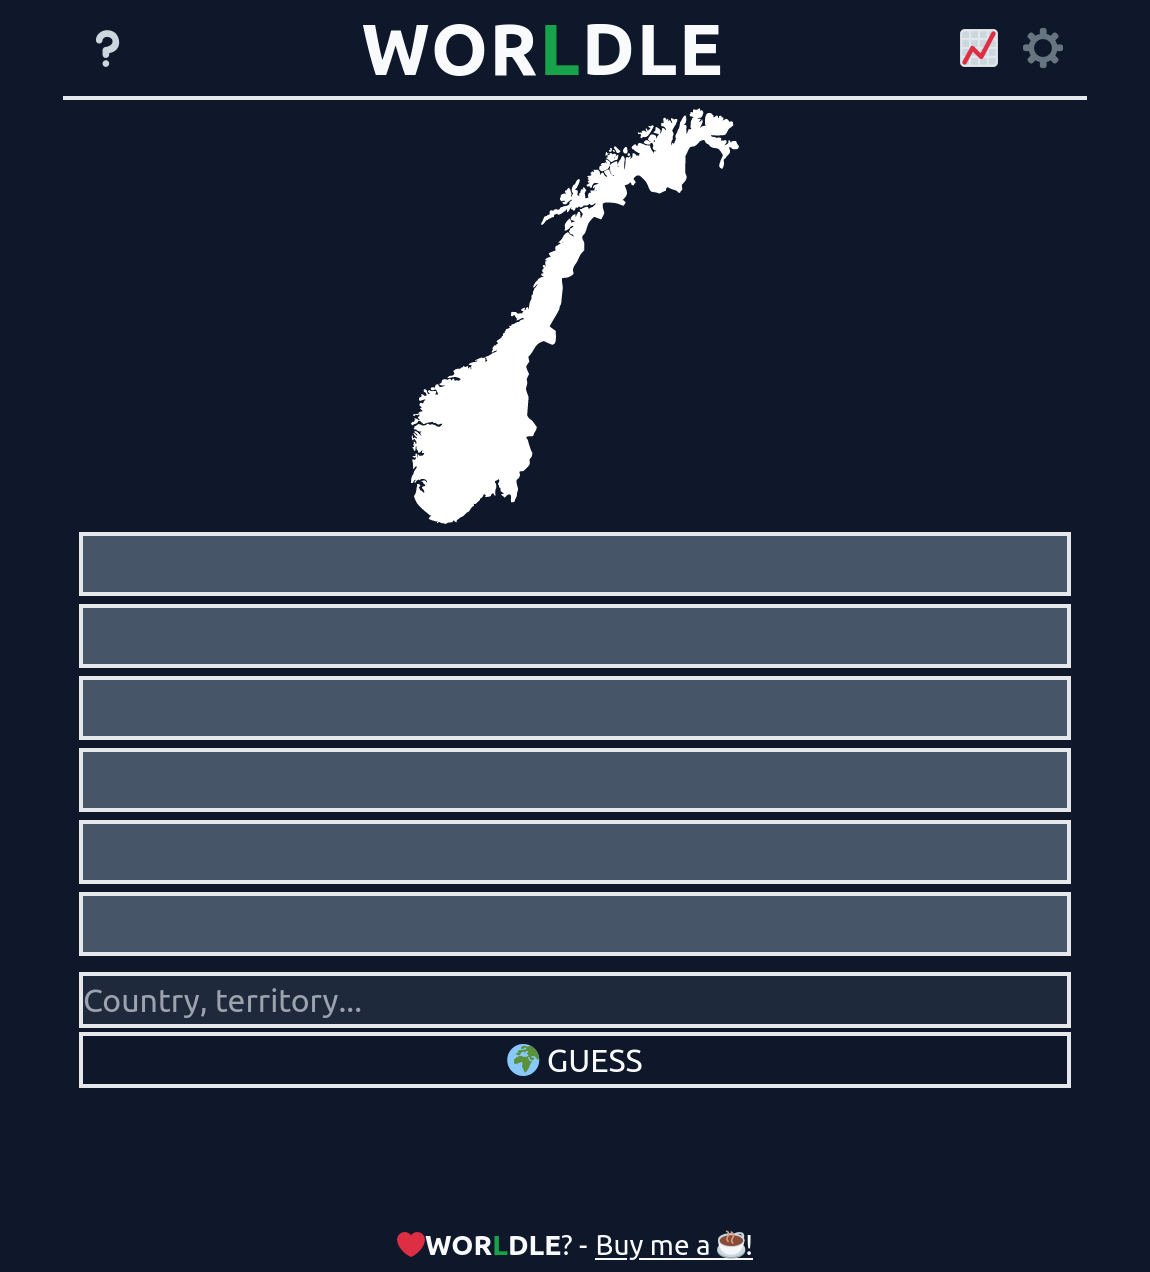
\includegraphics[height = 6cm]{images/otherGames/Worldle1.png}%
        }%
        \only<2>{%
        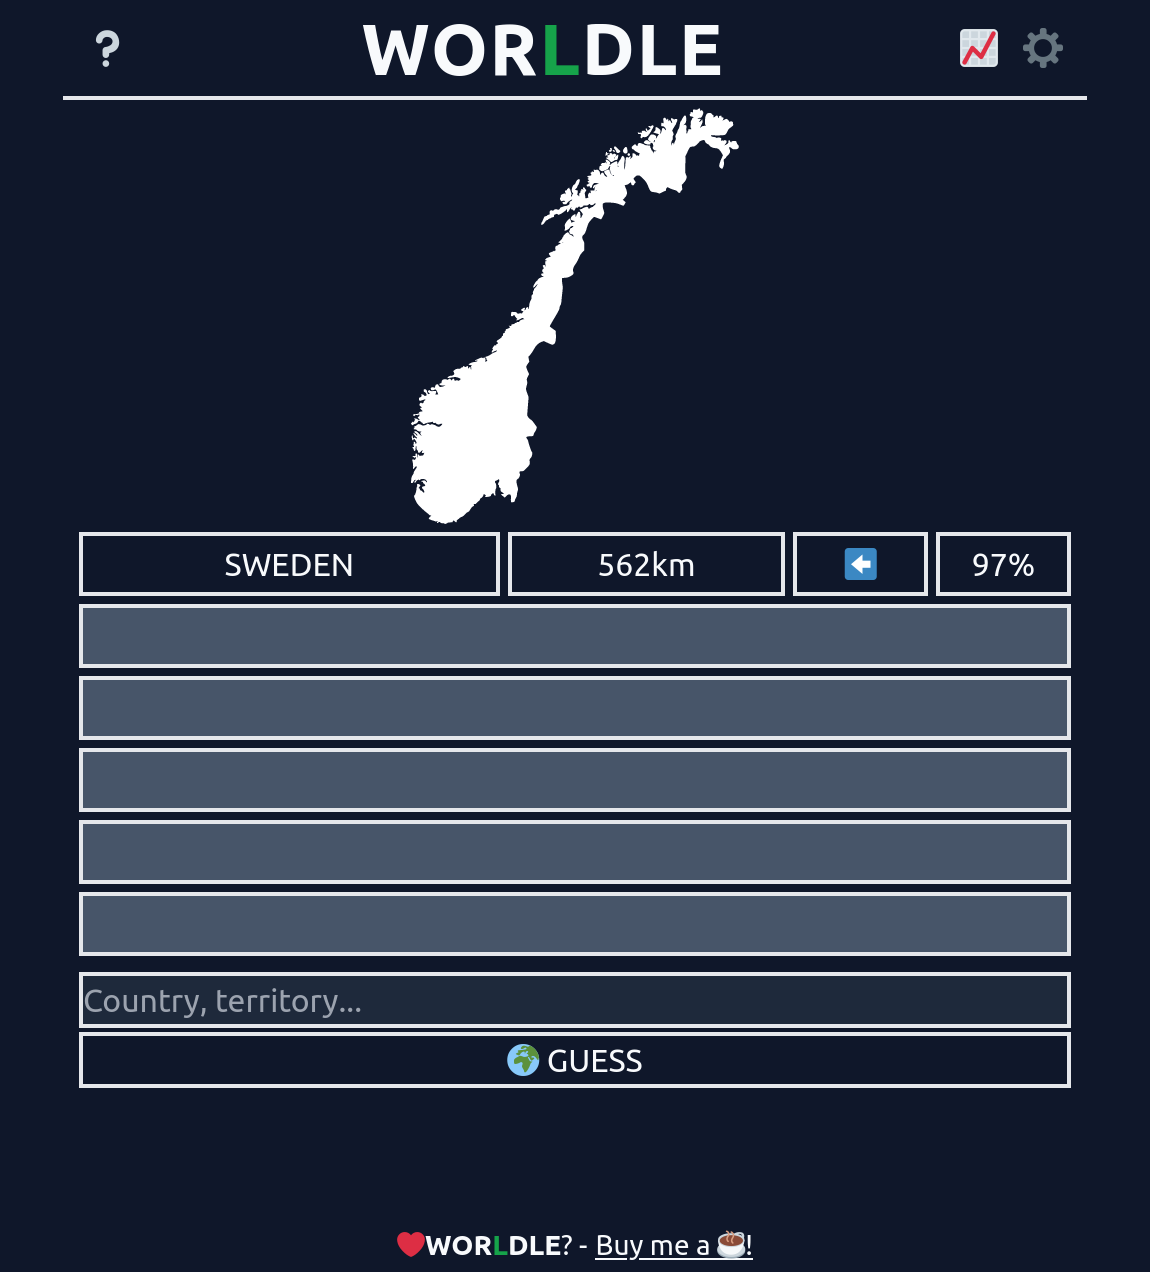
\includegraphics[height = 6cm]{images/otherGames/Worldle2.png}%
        }%
        \only<3>{%
        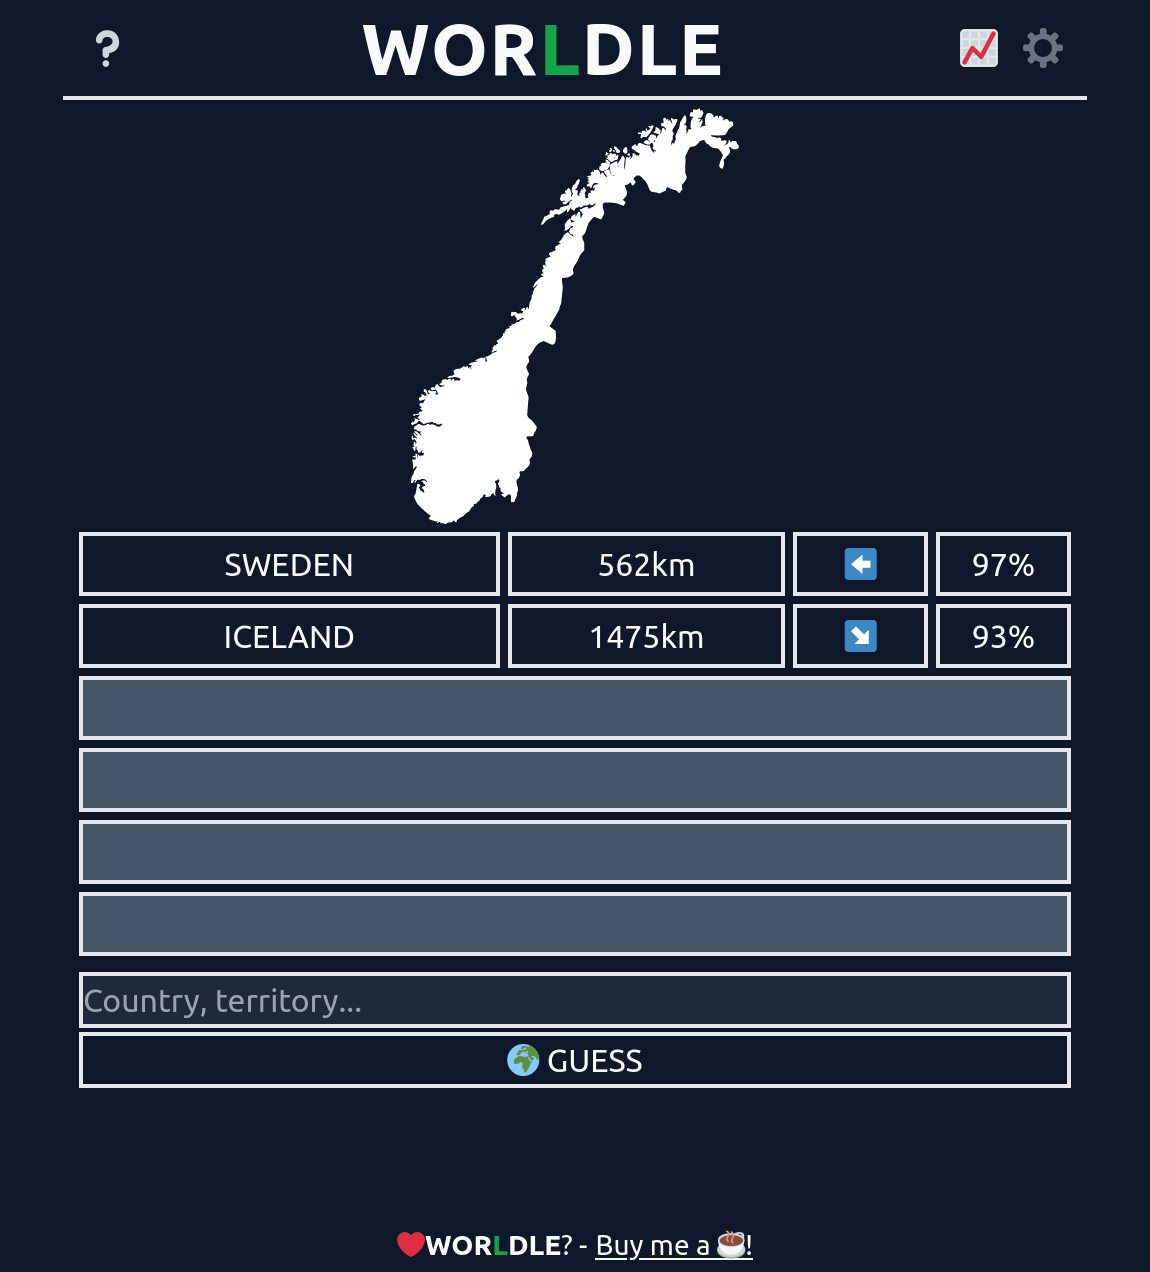
\includegraphics[height = 6cm]{images/otherGames/Worldle3.png}%
        }%
        \only<4>{%
        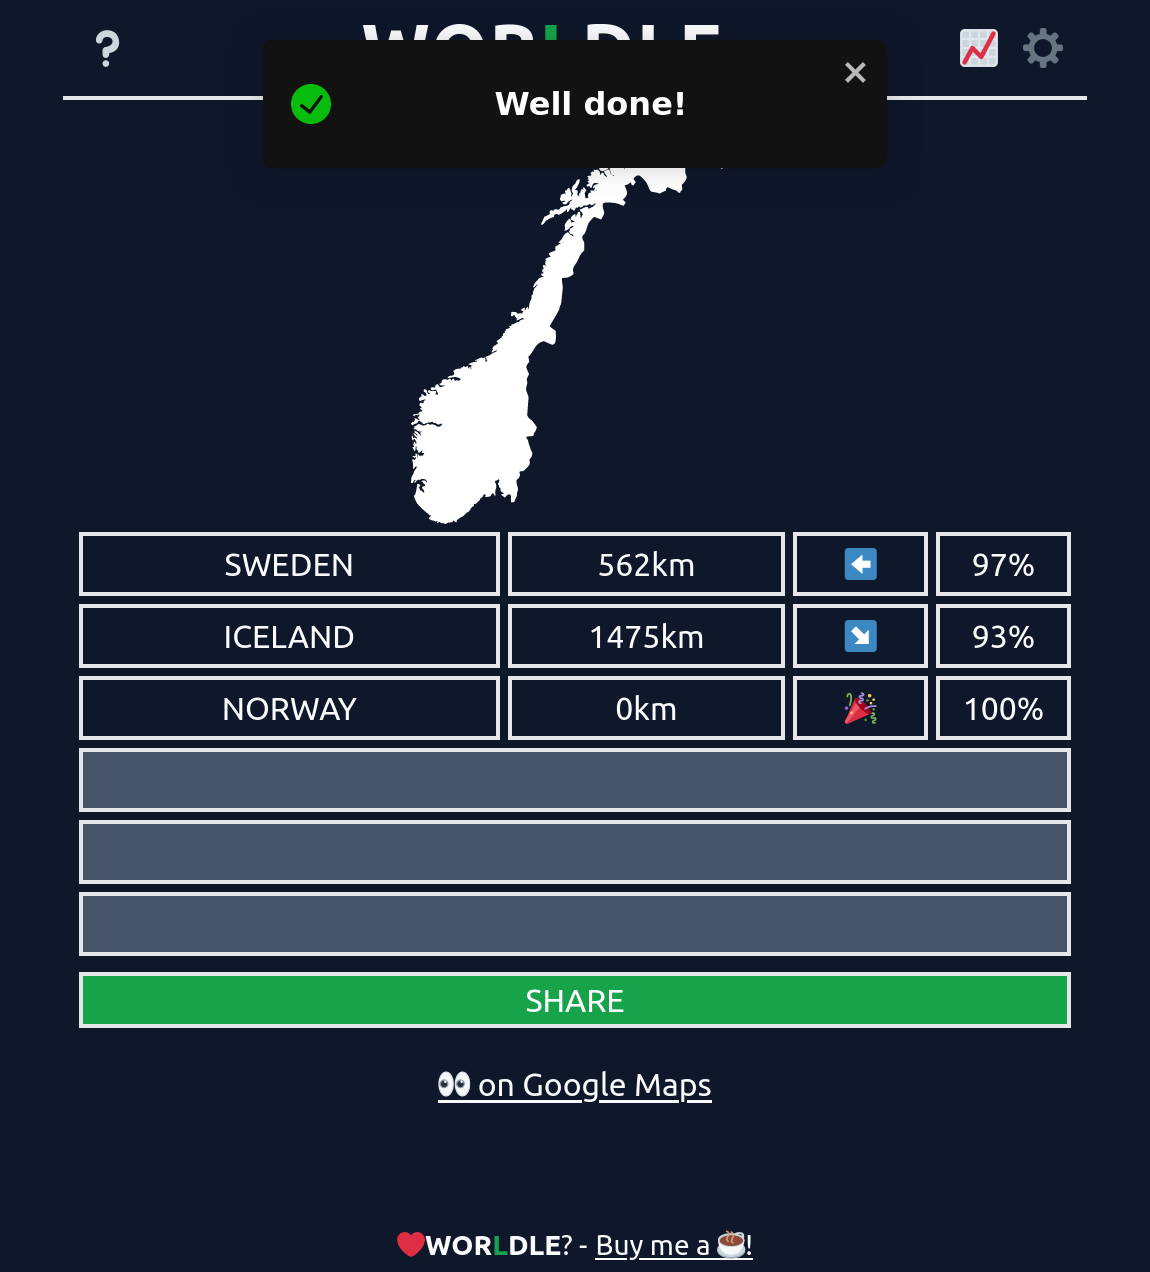
\includegraphics[height = 6cm]{images/otherGames/Worldle4.png}%
        }%
        \only<5>{%
        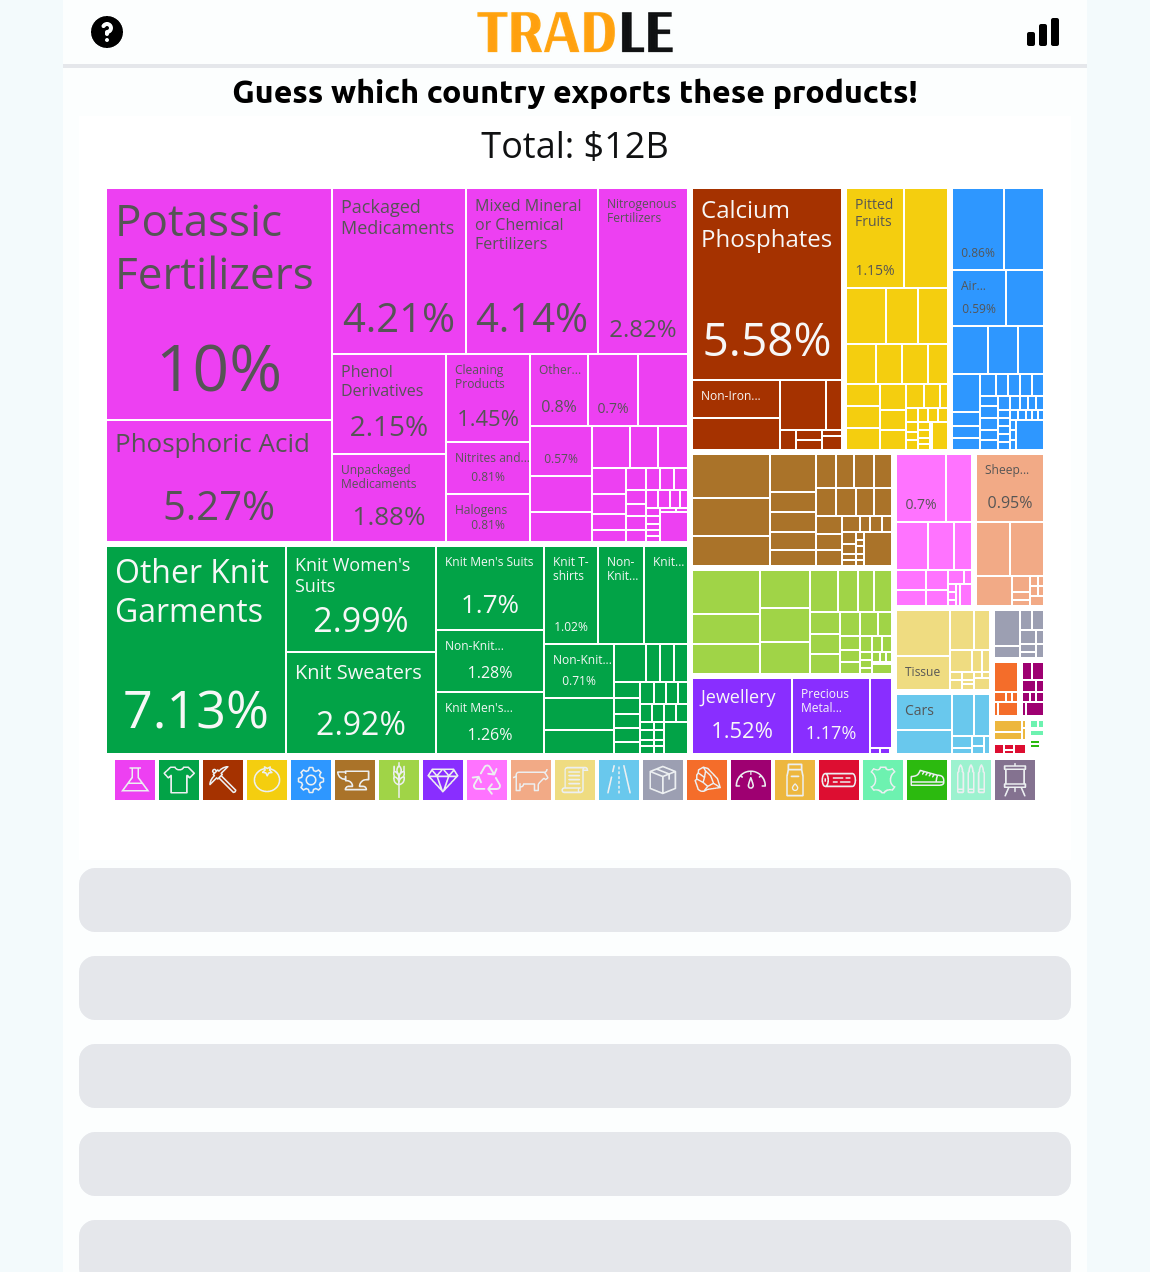
\includegraphics[height = 6cm]{images/otherGames/Tradle.png}%
        }%
        \only<6>{%
        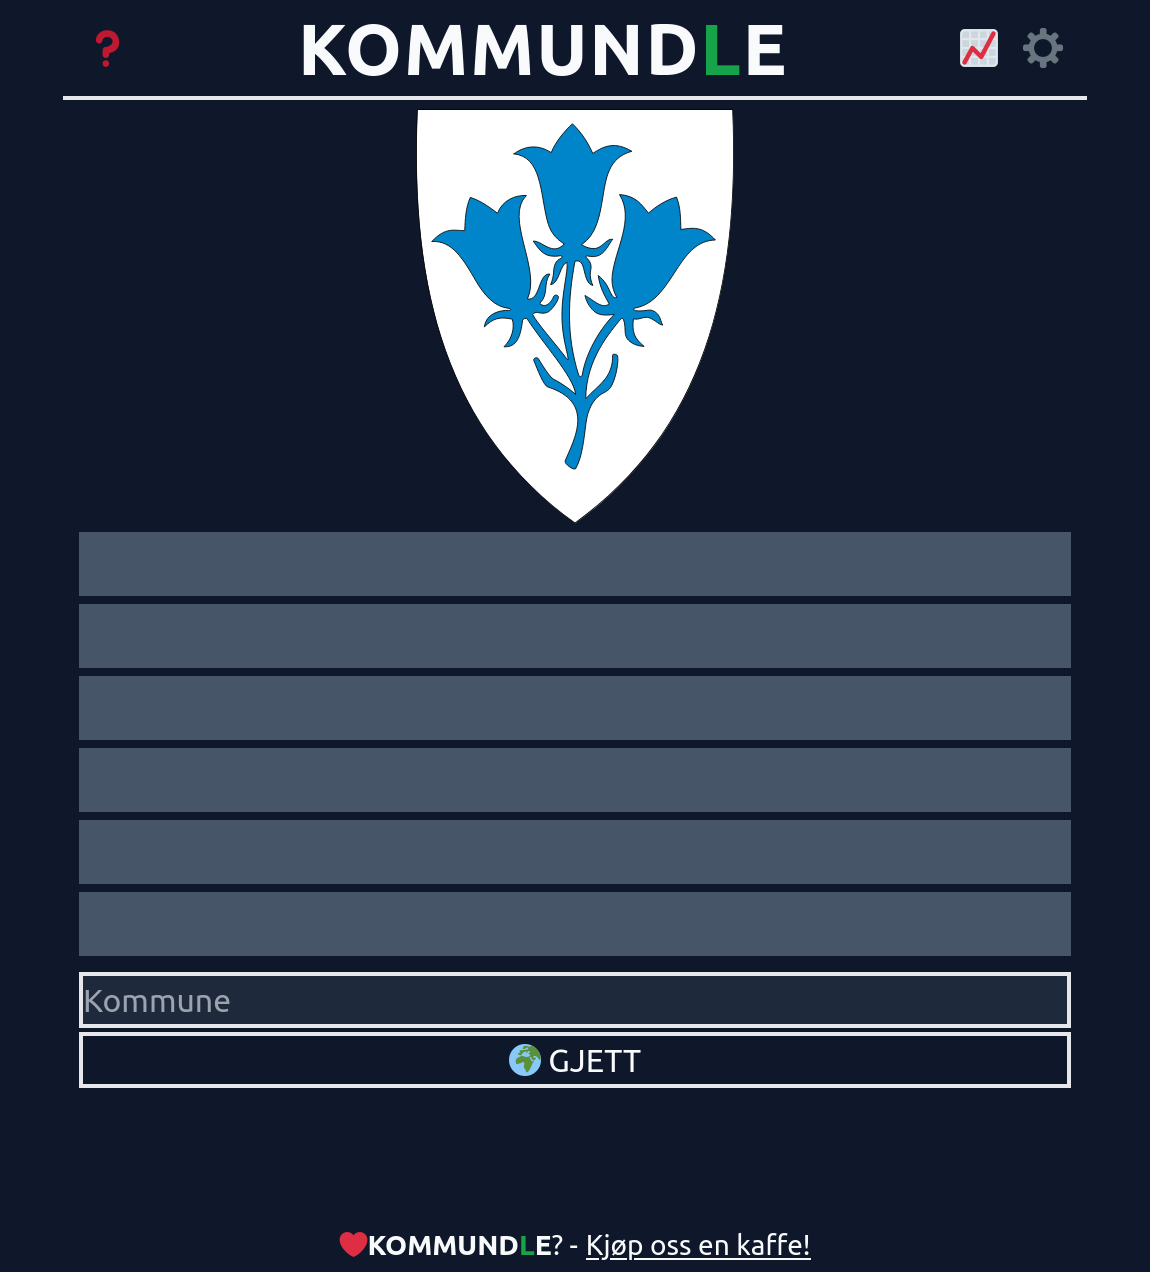
\includegraphics[height = 6cm]{images/otherGames/Kommundle.png}%
        }%
        \only<7>{%
        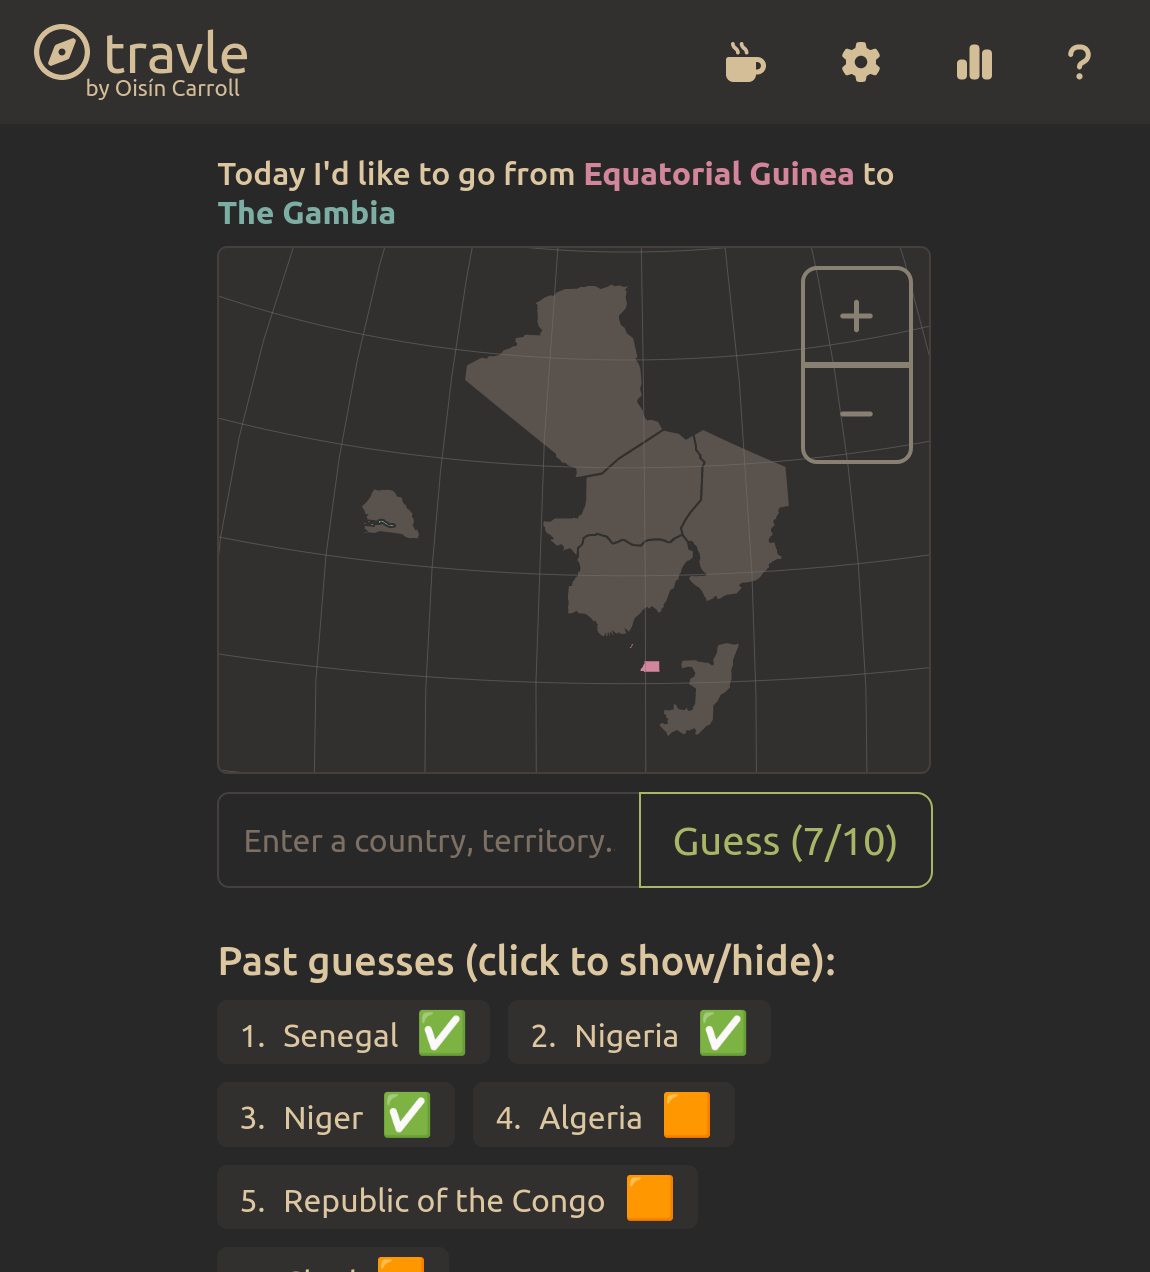
\includegraphics[height = 6cm]{images/otherGames/Travle.png}%
        }%
        \only<8>{%
        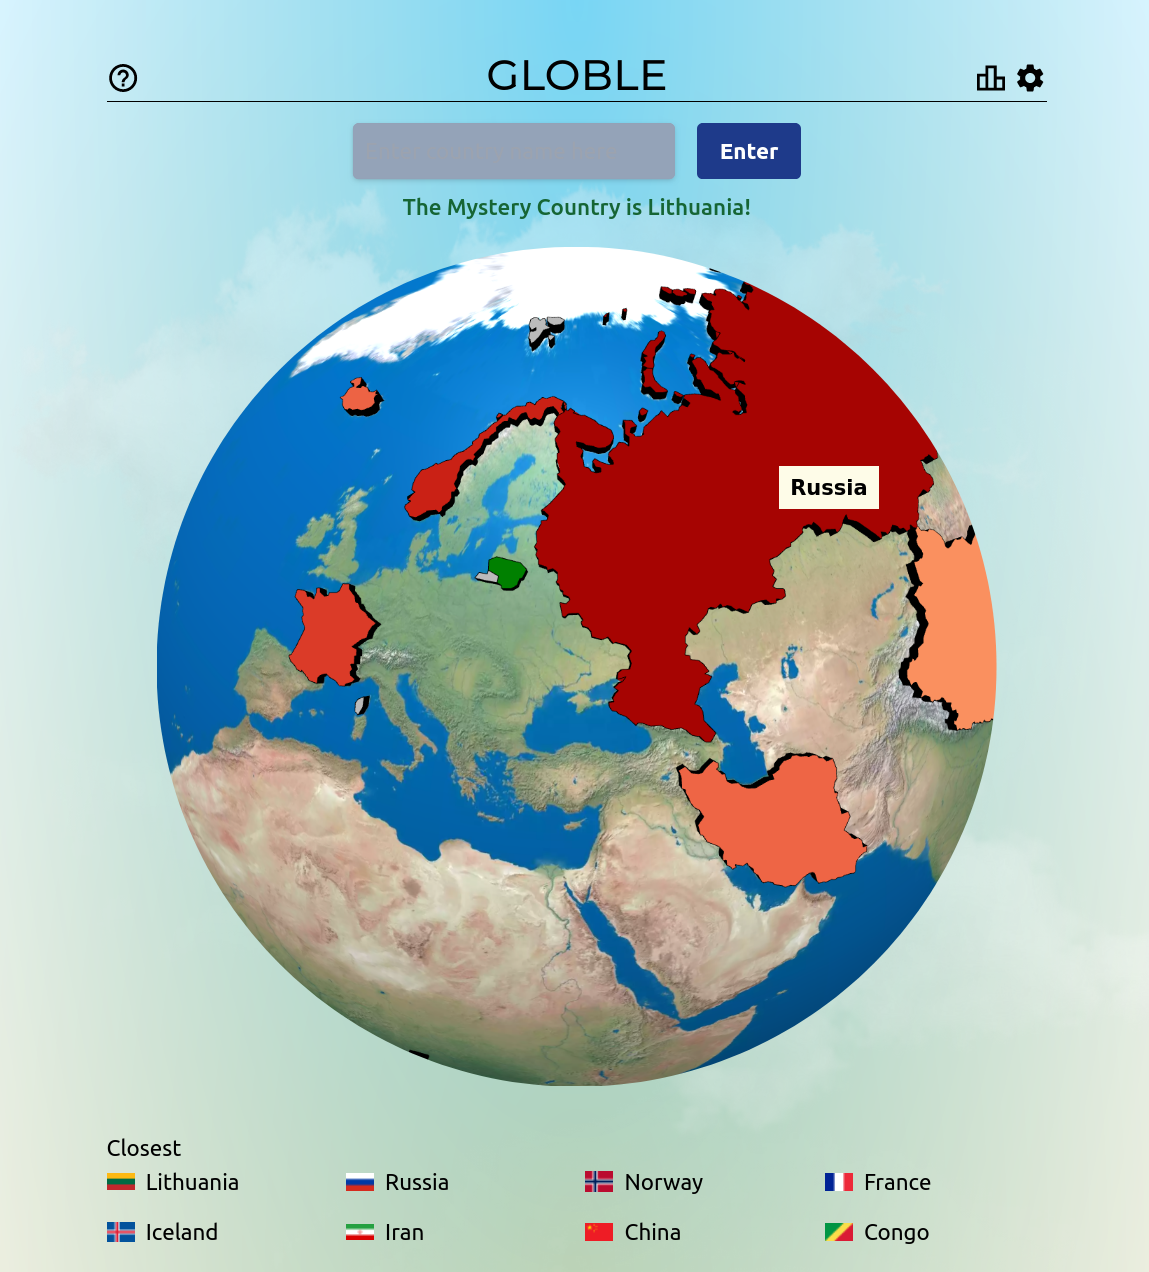
\includegraphics[height = 6cm]{images/otherGames/Globle.png}%
        }%

        %\caption{}
        \label{fig:worldle}
    \end{figure}

\end{frame}

\section{Guide to a terrible game}
\begin{frame}
    \begin{itemize}[<+->]
        \item Steal code from somebody else's project (Worldle)
        %\item Fjern all tull (React-frameworks, aggressiv linter, fransk oversettelse)
        \item Rewrite horrible code
        \item Remove fuzz (French, light mode)
        \item Insert a passive aggressive FAQ with Bergen-jokes
        \item Data???
        \item What is an area, district or whatever?
        \item What are Fantoft, Bryggen or Loddefjord?
        \item Where are the borders of all of these?
    \end{itemize}
\end{frame}

\begin{frame}
    \begin{block}{Kartverk}
        %\enquote{Vi har tidligere prøvd å kartlegge strøk i Bergen. Utfordringen den gang var at det var mange innspill og meninger om hvor de forskjellige grensene gikk for strøkene. Det ble ikke realisert siden bergensere ikke hadde godkjent en løsning.}
        %\enquote{Vi har tidligere prøvd å kartlegge strøk i Bergen. Utfordringen var at det var mange innspill og meninger om hvor de forskjellige grensene gikk. Det ble ikke realisert siden bergensere ikke hadde godkjent en løsning.}
        \enquote{We have previously tried to map neighbourhoods in Bergen. The challenge was that there was a lot of input and opinions about where the different boundaries went. It wasn't realised because the people of Bergen hadn't approved a solution.}
    \end{block}
    \pause
    \begin{block}{Kartverk}
        %\enquote{Men det er ingenting i veien for at du selv kan digitalisere din egen versjon av Bergen. For å hjelpe deg har jeg laget en liten veiledning på hvordan dette kan gjøres.}
        %\enquote{Men det er ingenting i veien for at du selv kan digitalisere din egen versjon av Bergen. For å hjelpe deg har jeg laget en liten veiledning på hvordan dette kan gjøres.}
        \enquote{But there's nothing to stop you from digitising your own version of Bergen. To help you out, I've created a little guide on how this can be done.}
    \end{block}
    %\pause
    %\begin{block}{Stackoverflow}
    %    \enquote{Of course you have to use the EPSG:25832 projection for the type of project you are working with.}
    %\end{block}
\end{frame}

\section{Qgis}
\begin{frame}
    \begin{figure}
        \centering
        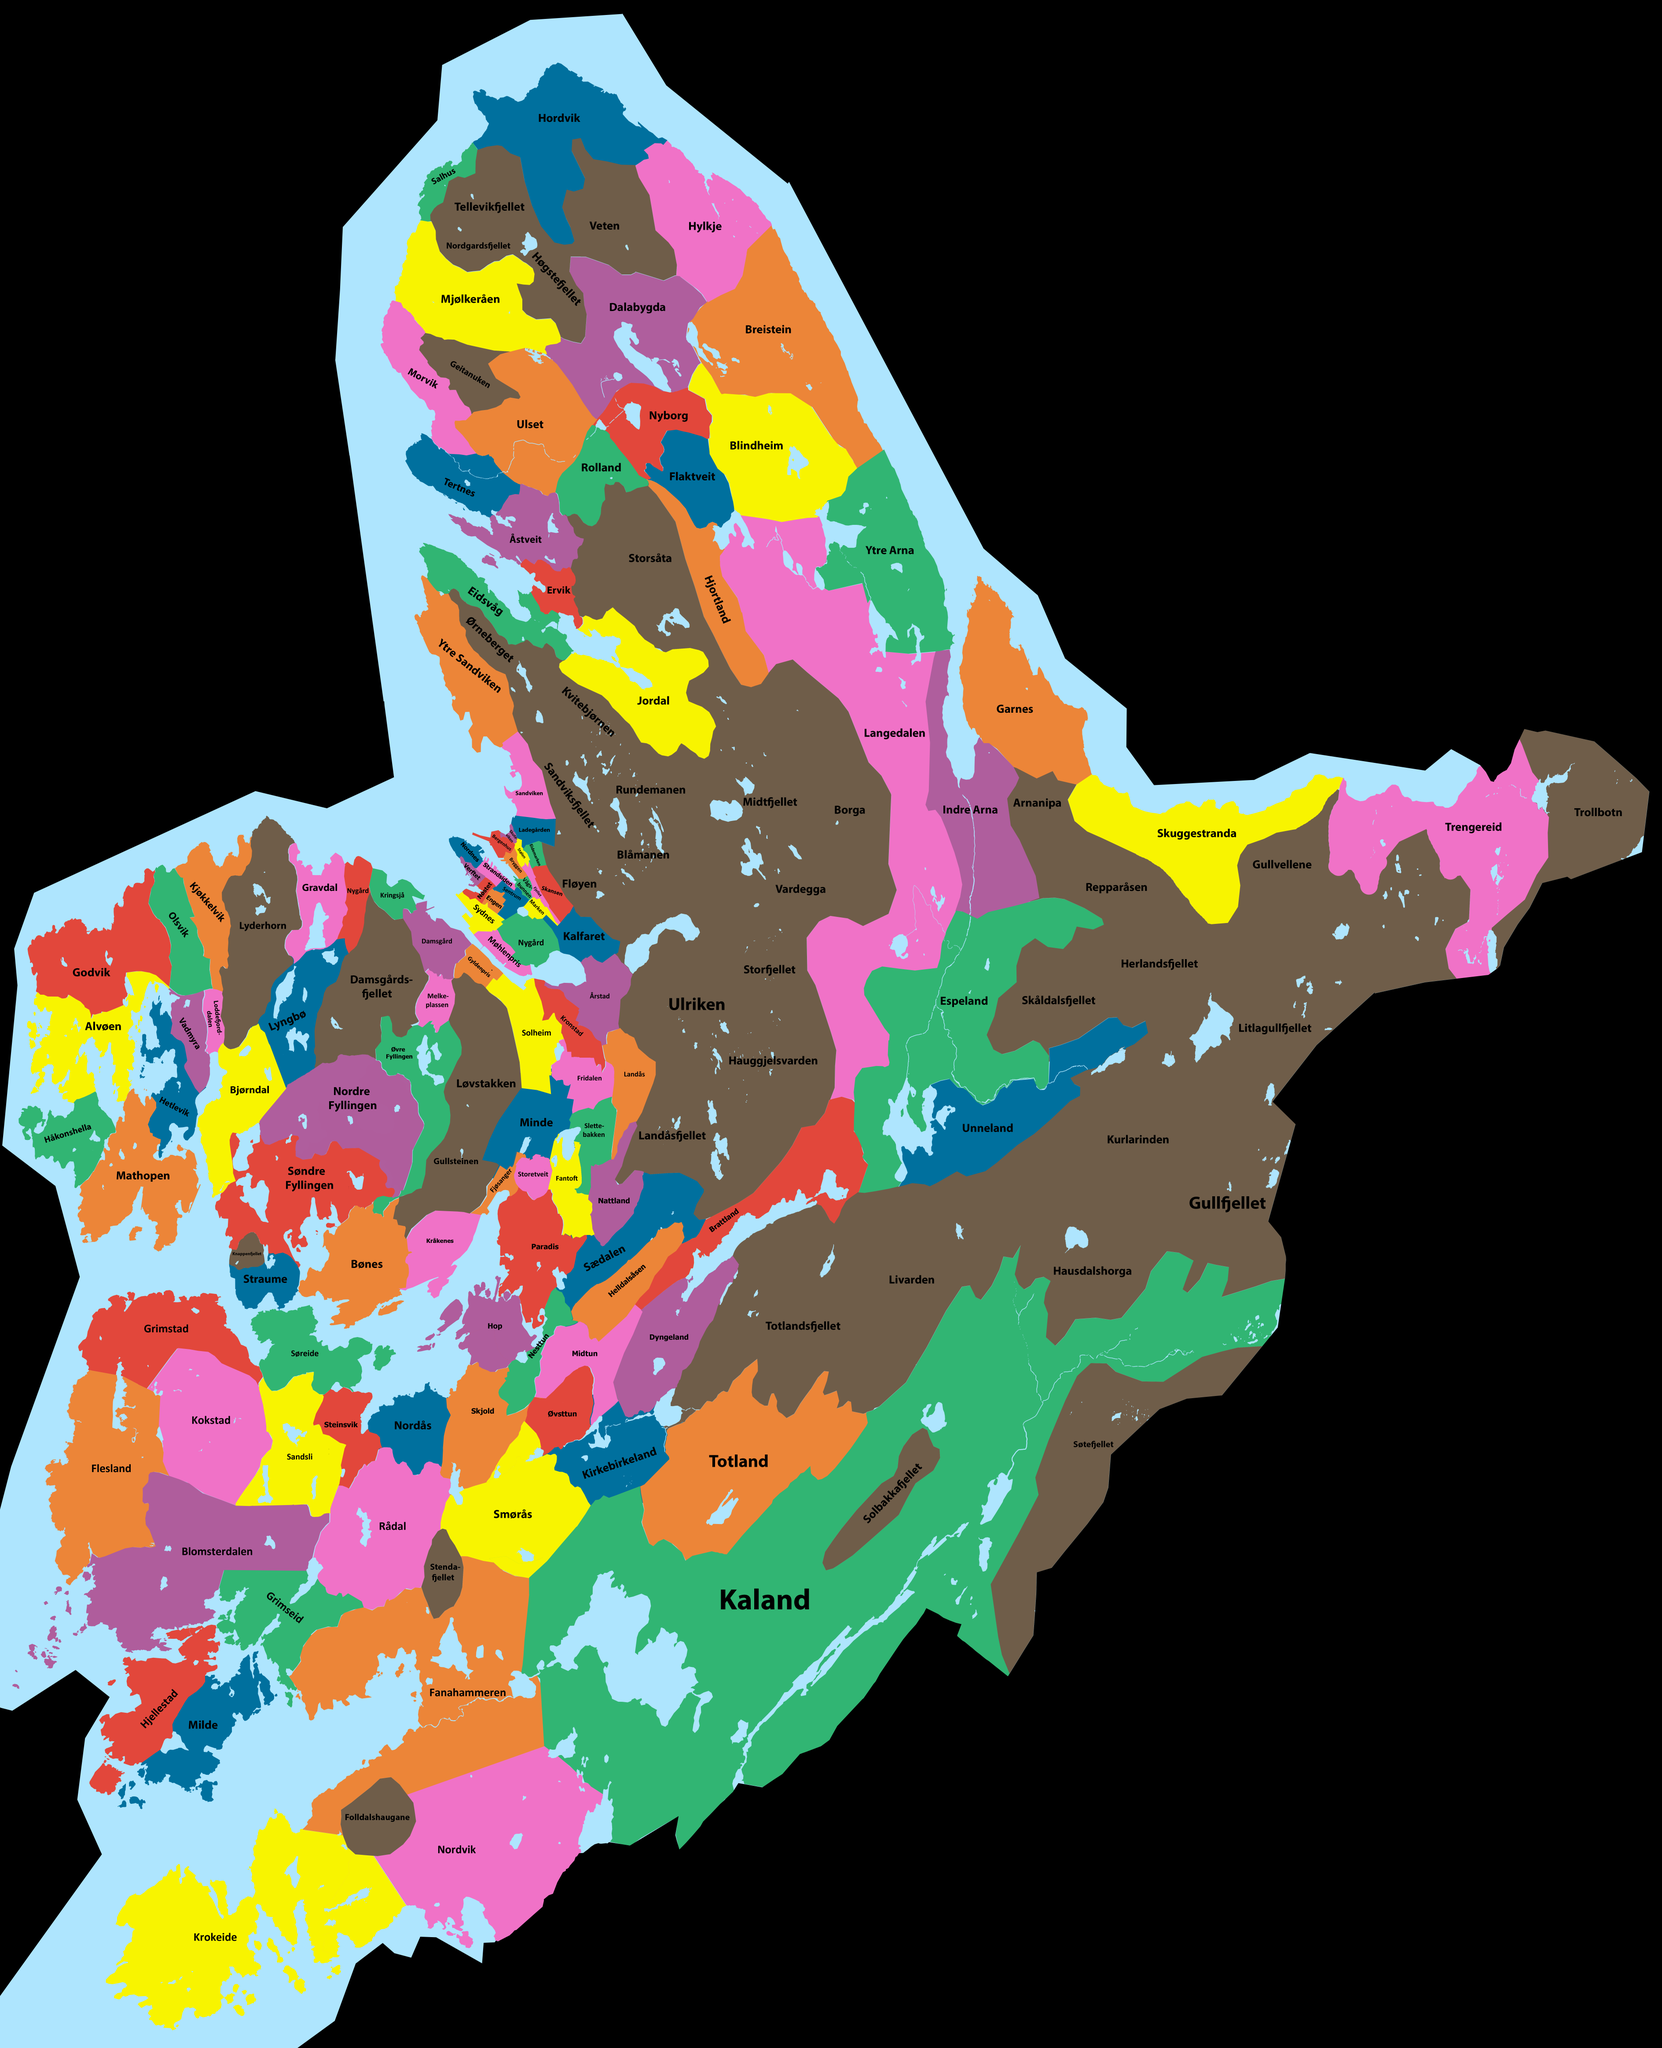
\includegraphics[height = 6cm]{images/boligomraaderWiki.png}%
        \caption{Geography of Bergen - The truth}
    \end{figure}
\end{frame}

\begin{frame}
    \begin{itemize}[<+->]
        \item Original is a PNG file, not SVG
        \item $\Rightarrow$ Contact author about data source
        \item $\Rightarrow$ No answer
        \item Try to unassemble by using different tools (AI sucks)
        \item $\Rightarrow$ No success
    \end{itemize}
\end{frame}

\begin{frame}
    \begin{figure}
        \centering
        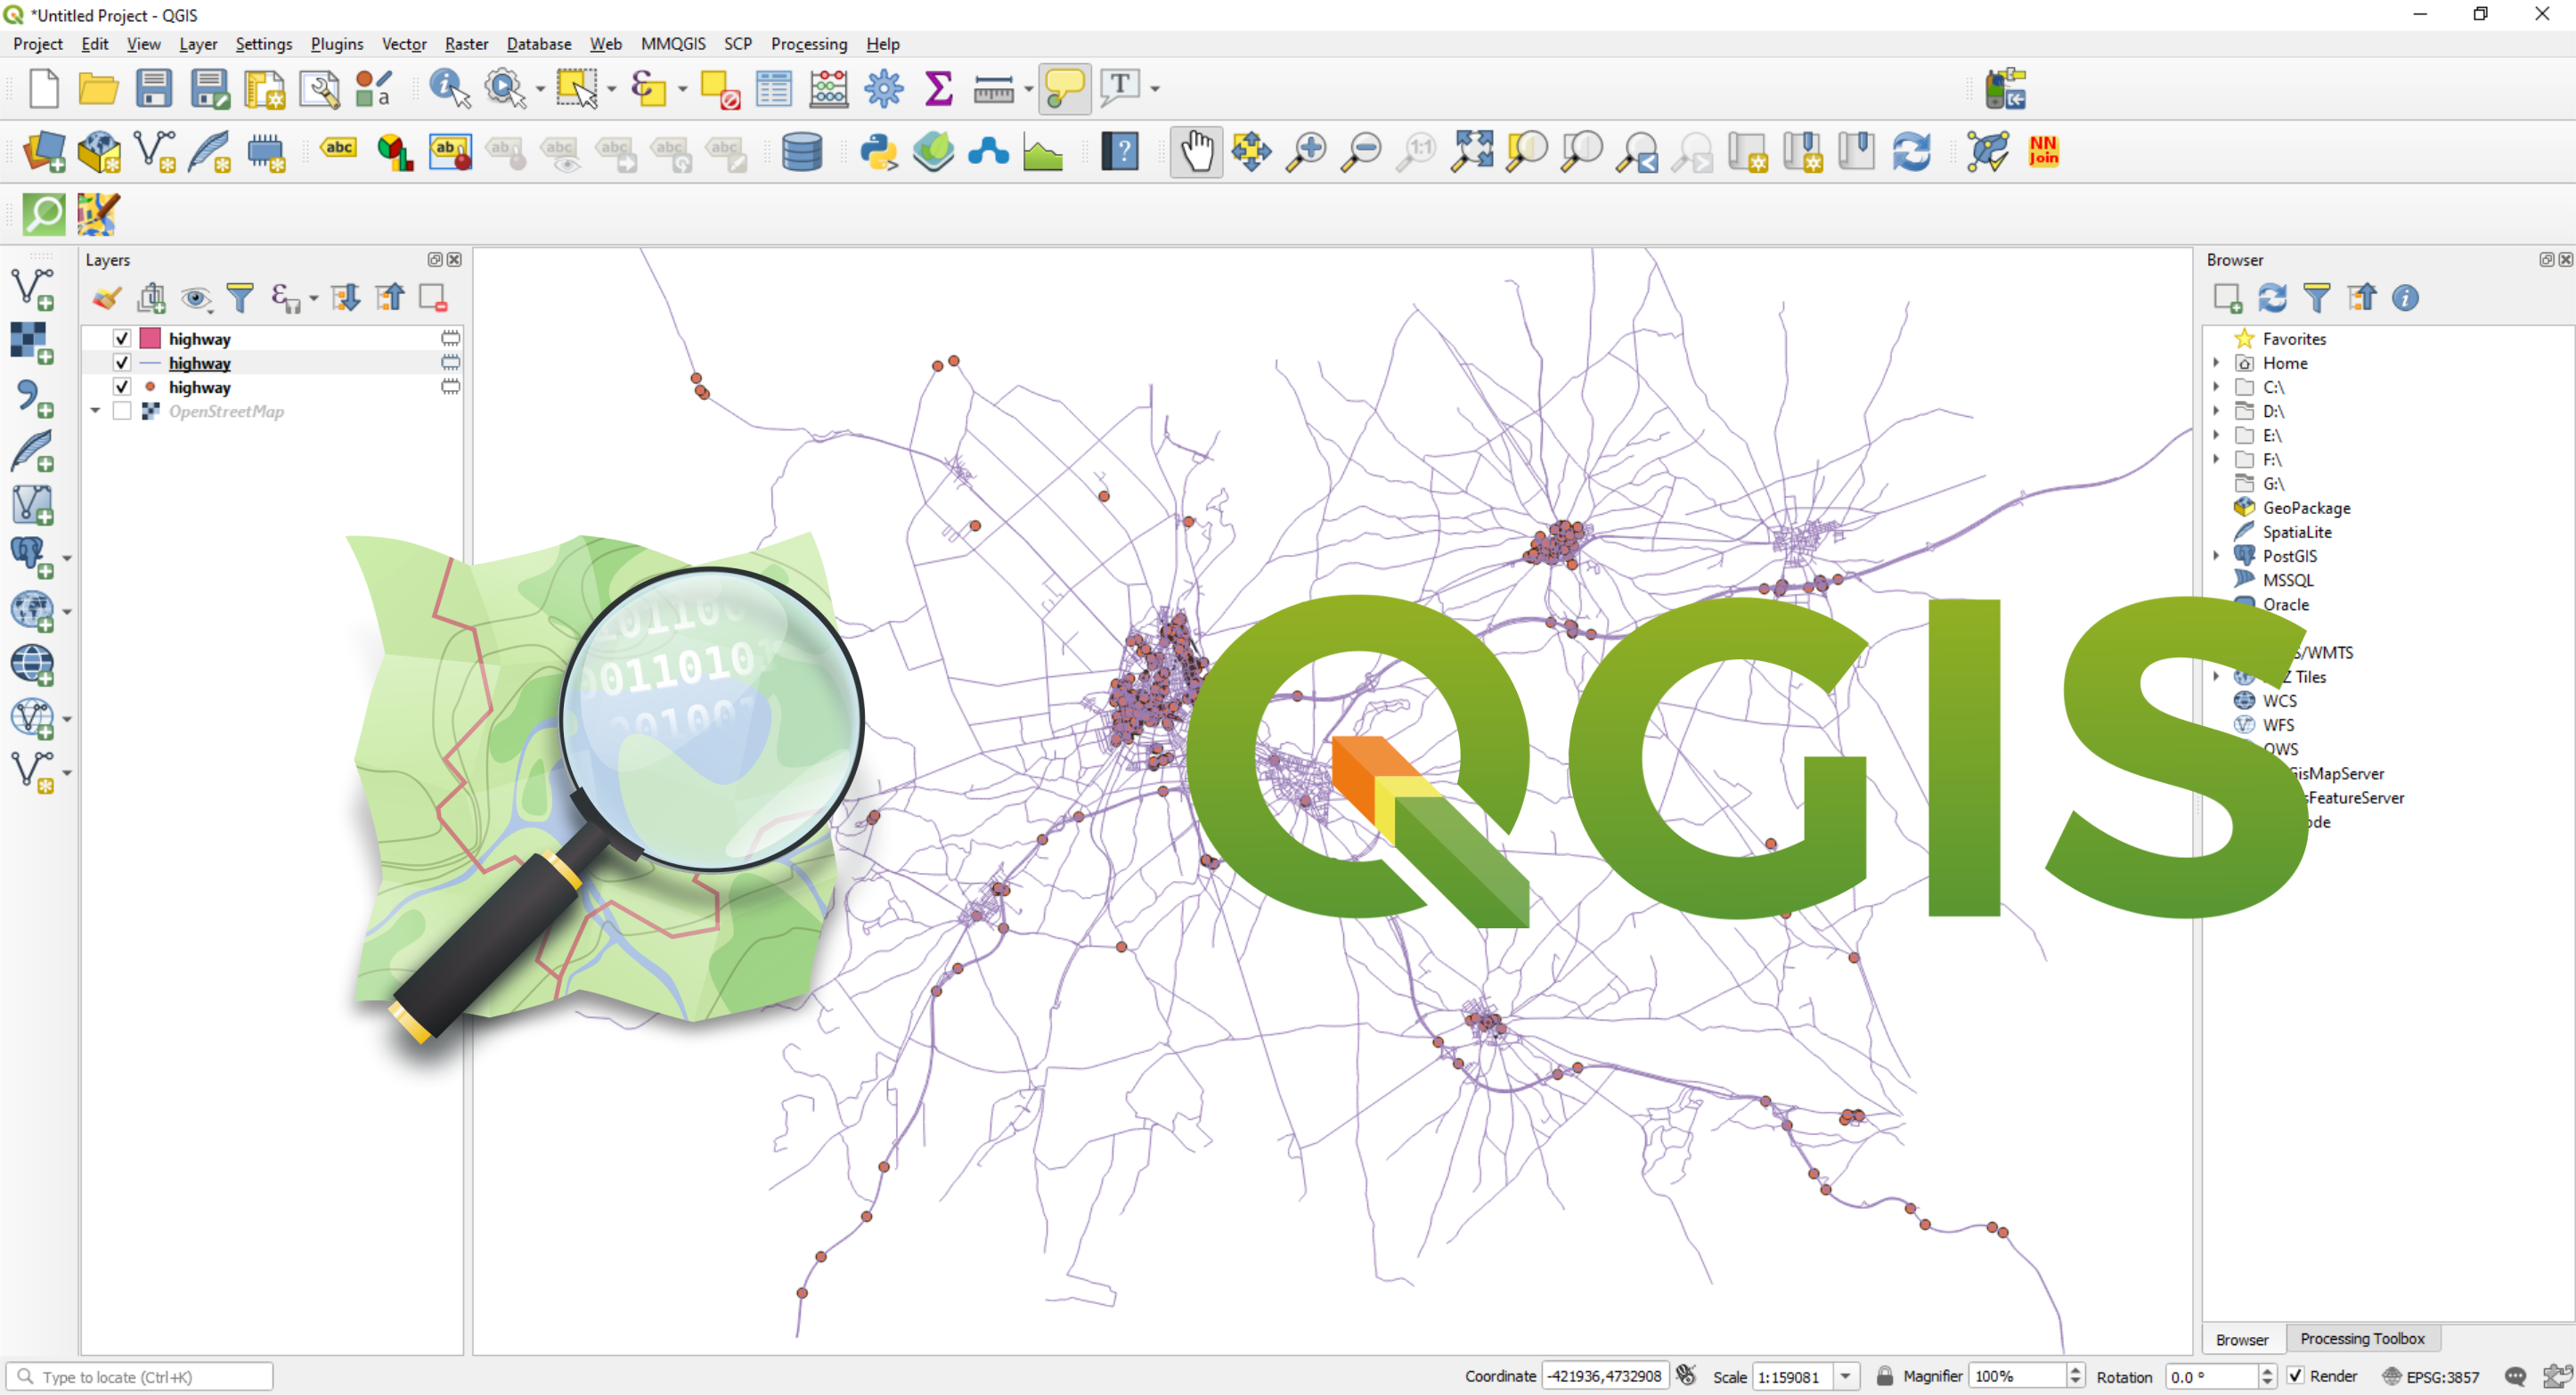
\includegraphics[height = 6cm]{images/qgis.png}%
        \caption{Qgis - A programme of horror}
    \end{figure}
\end{frame}

\begin{frame}{Settings}
    \begin{itemize}[<+->]
        \item Click through six pages of settings to set up a project
        \item Let's learn 5 years of cartography studies in one hour
        \item Projection? Mercator?
        \pause
        \begin{block}{Stackoverflow}
            \enquote{Of course you have to use the EPSG:25832 projection for the type of project you are working with.}
        \end{block}
    \end{itemize}
\end{frame}

\begin{frame}
    \begin{figure}
        \centering
        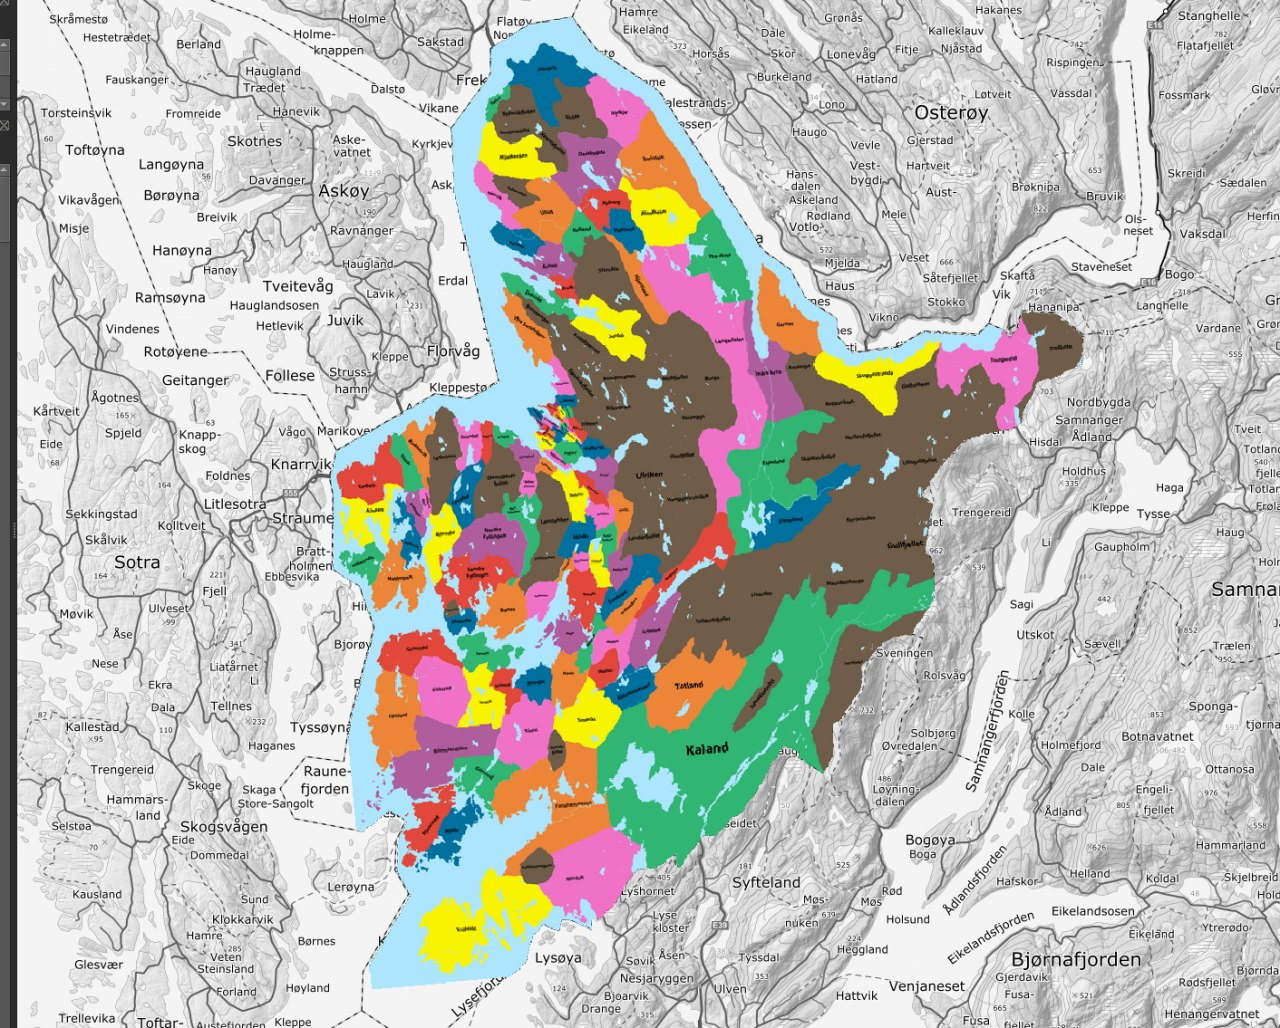
\includegraphics[height = 6cm]{images/qgis1.jpg}%
        \caption{Initialise correct layers}
    \end{figure}
\end{frame}

\begin{frame}
    \begin{figure}
        \centering
        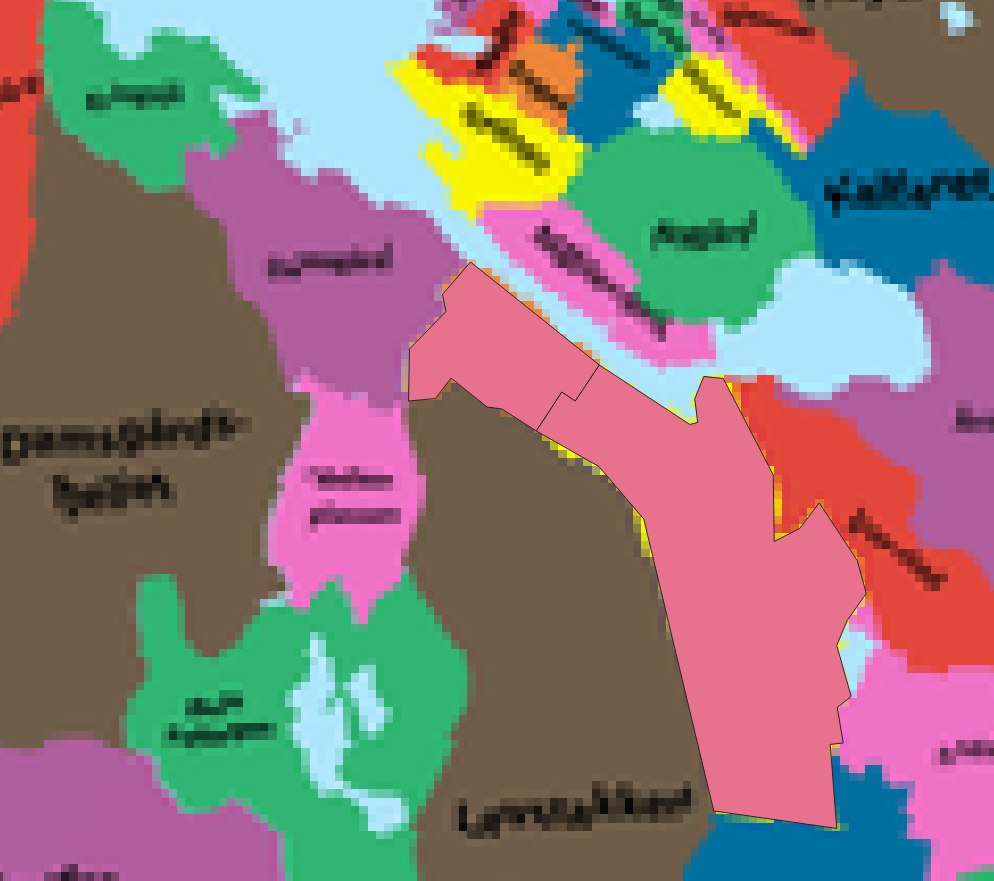
\includegraphics[height = 6cm]{images/qgis2.png}%
        \caption{Draw some borders}
    \end{figure}
\end{frame}

\begin{frame}
    \begin{figure}
        \centering
        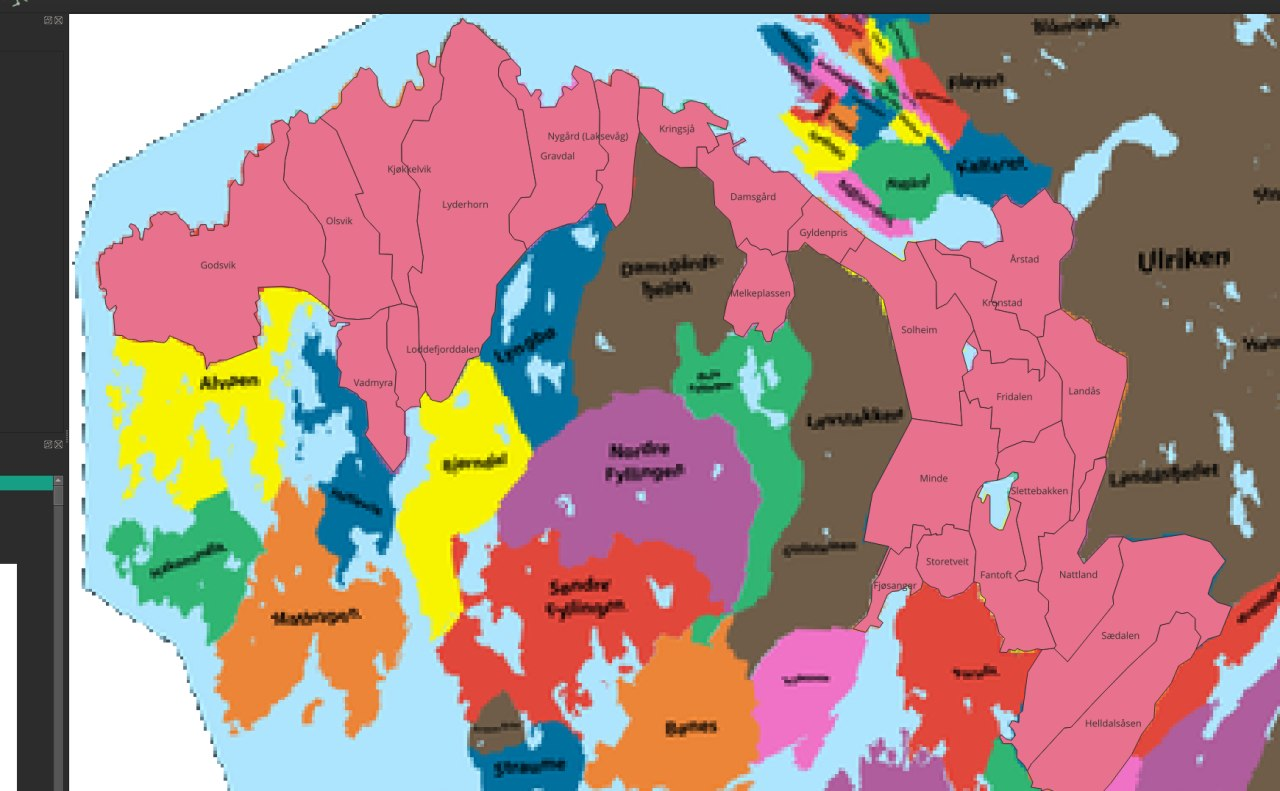
\includegraphics[height = 6cm]{images/qgis3.jpg}%
        \caption{More drawing}
    \end{figure}
\end{frame}

\begin{frame}
    \begin{figure}
        \centering
        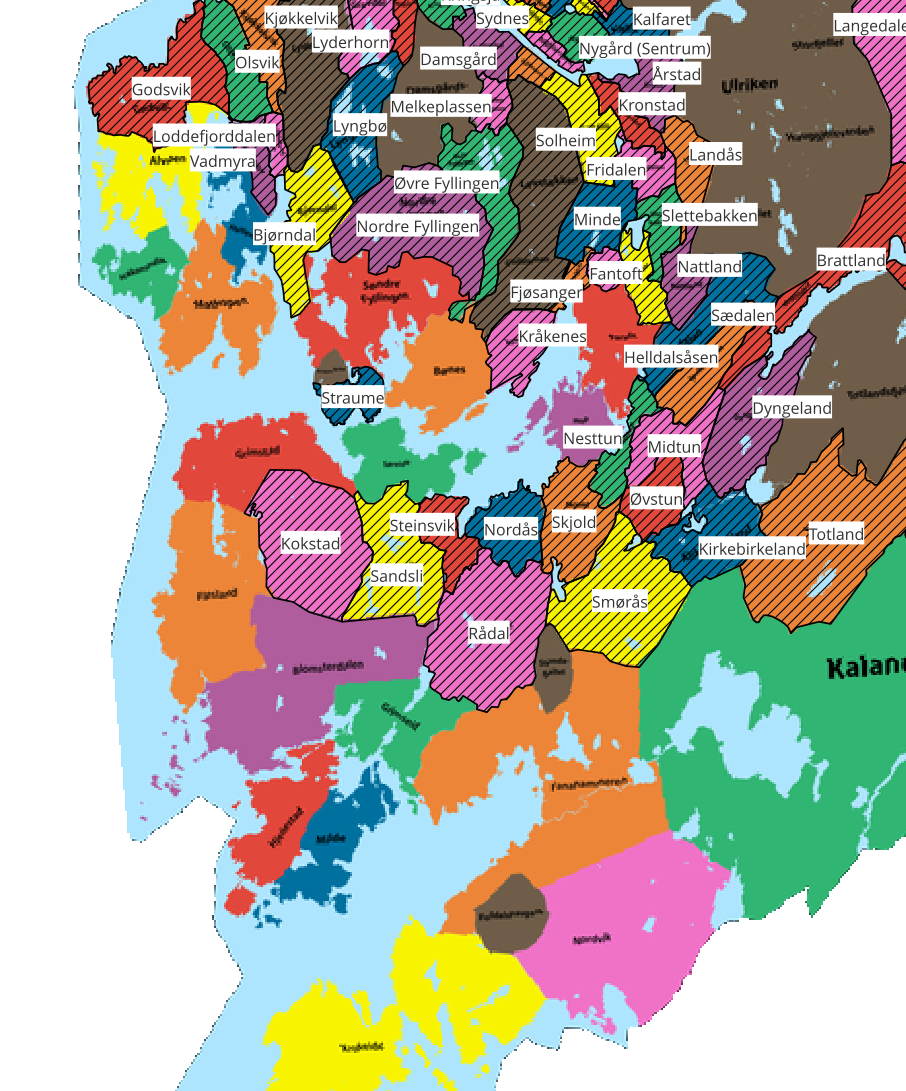
\includegraphics[height = 6cm]{images/qgis4.png}%
        \caption{Even more drawing}
    \end{figure}
\end{frame}

%\begin{frame}
%    \begin{figure}
%        \centering
%        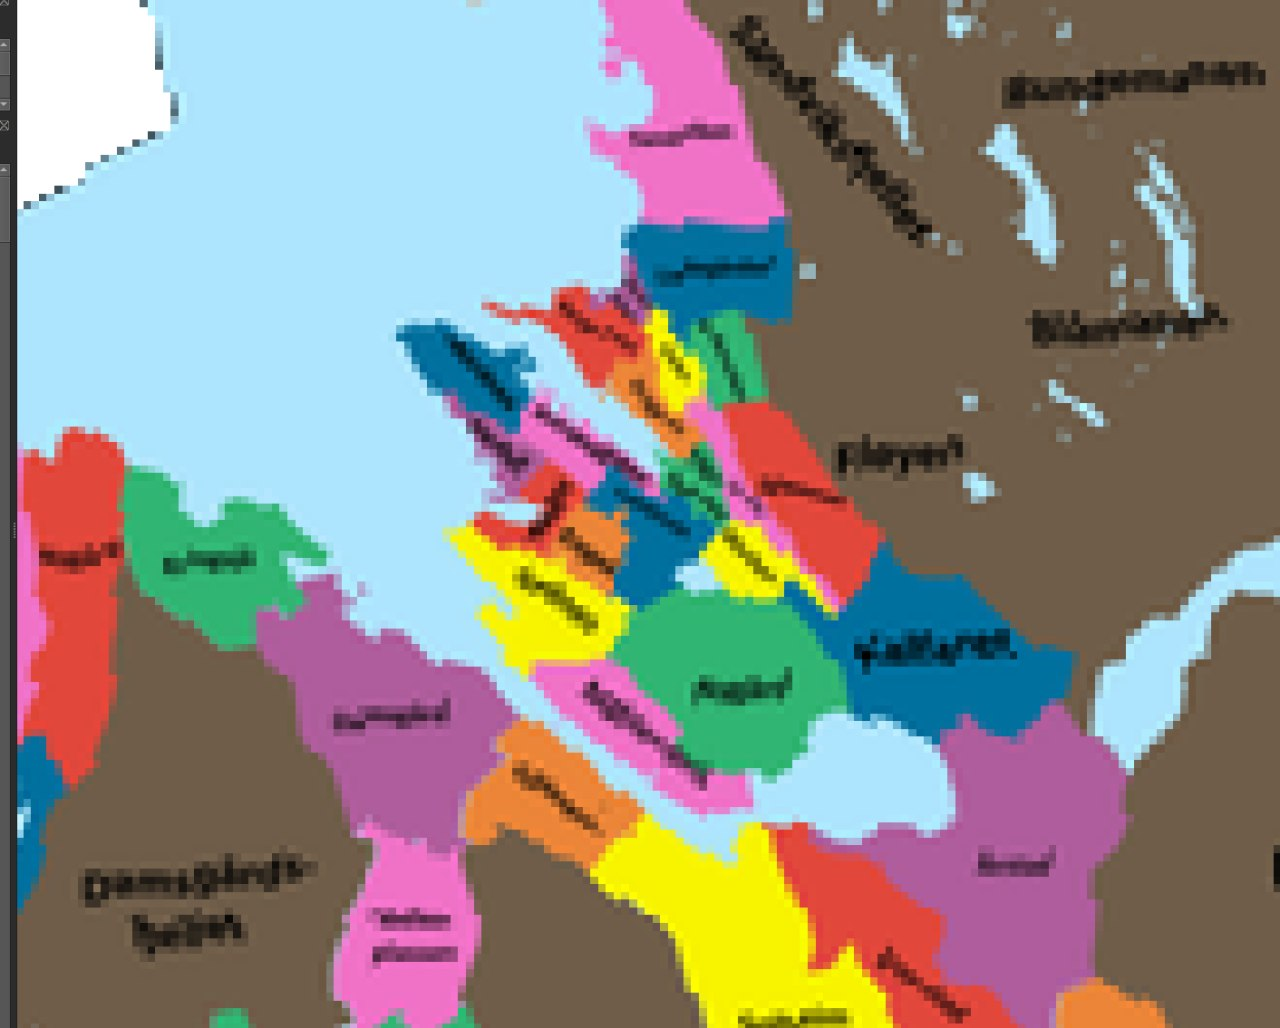
\includegraphics[height = 6cm]{images/qgis5.png}%
%        \caption{Sentrum???}
%    \end{figure}
%\end{frame}

\begin{frame}
    \begin{figure}
        \centering
        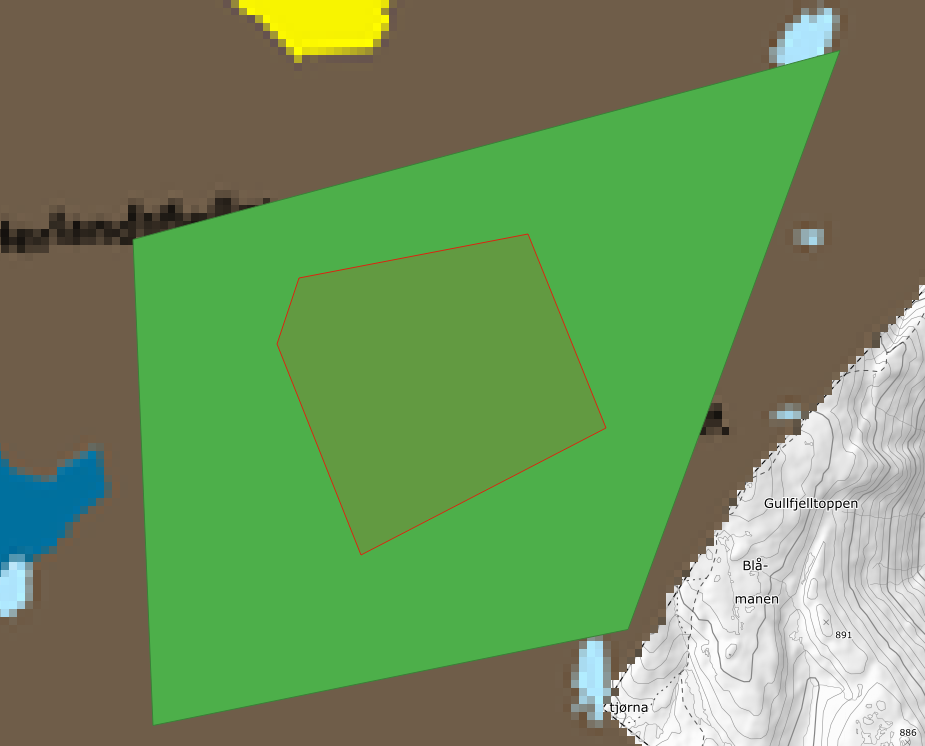
\includegraphics[height = 6cm]{images/qgis_shapeInShape.png}%
        \caption{Lakes? \enquote{The inserted ring is not contained in the other ring.}}
    \end{figure}
\end{frame}

%\begin{frame}
%   \begin{figure}
%        \centering
%        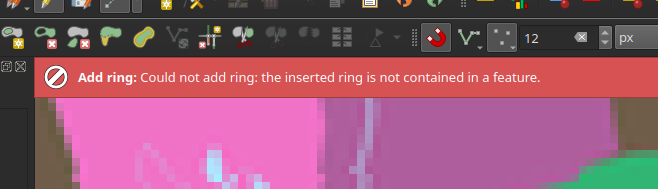
\includegraphics[height = 4cm]{images/qgis_ringInRing.png}%
%        \caption{Er EPSG:25832 det man ser?}
%    \end{figure}
%\end{frame}

\begin{frame}
    \begin{figure}
        \centering
        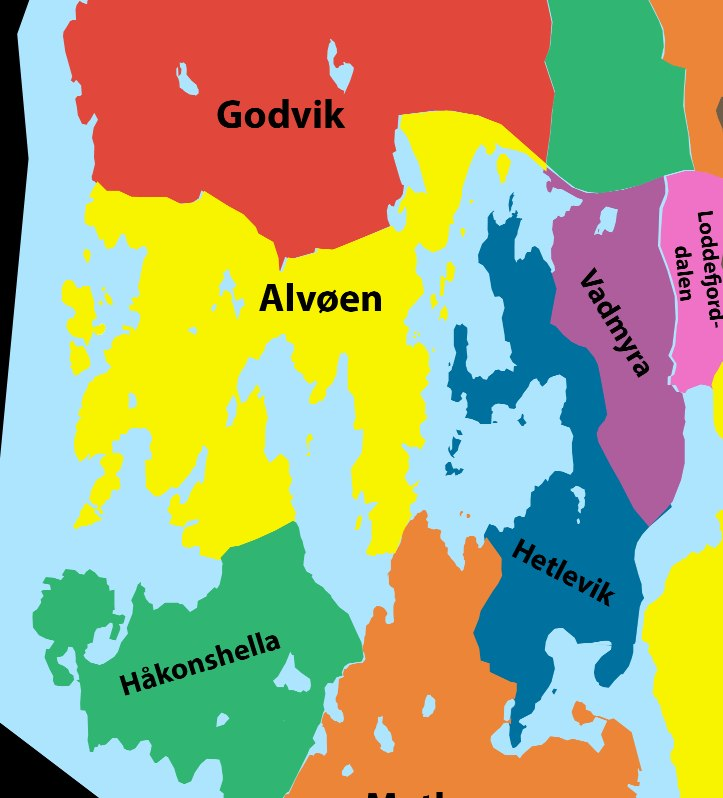
\includegraphics[height = 6cm]{images/qgis_islands.jpg}%
        \caption{Islands? \enquote{Could not add multi part element. This layer (type multilayer) does not support multi layer elements.}}
    \end{figure}
\end{frame}

\begin{frame}
    \begin{figure}
        \centering
        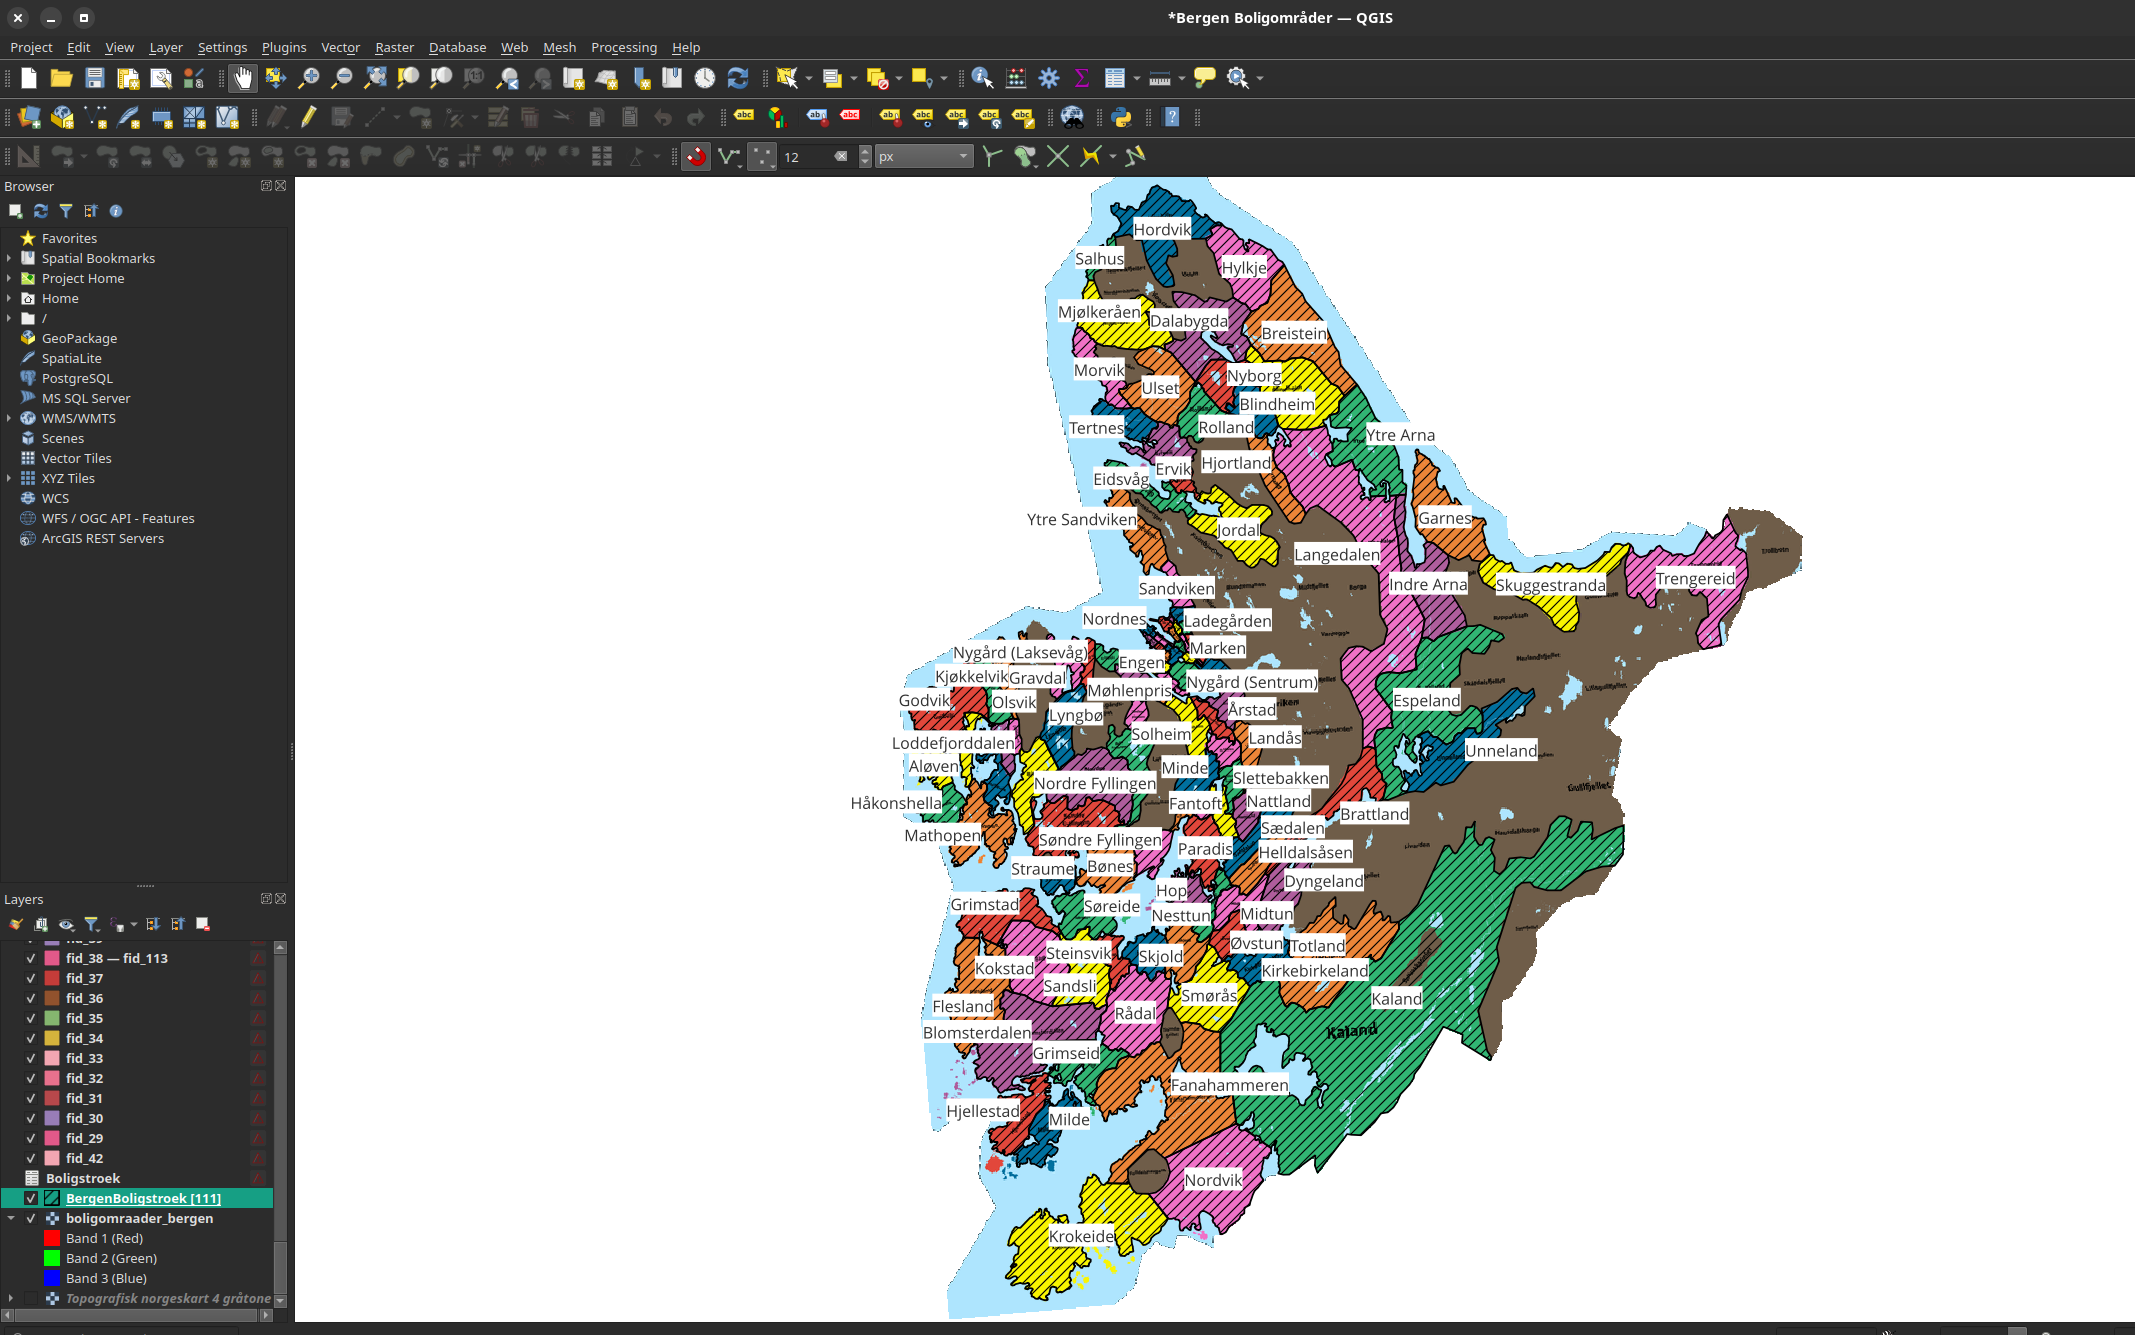
\includegraphics[height = 6cm]{images/qgisOverview.png}%
        \caption{Finally}
    \end{figure}
\end{frame}

%\begin{frame}
%    \begin{alertblock}{Error}
%        \enquote{Could not add multi part element. This layer (type multilayer) does not support multi layer elements.}
%    \end{alertblock}
%    \begin{figure}
%        \centering
%        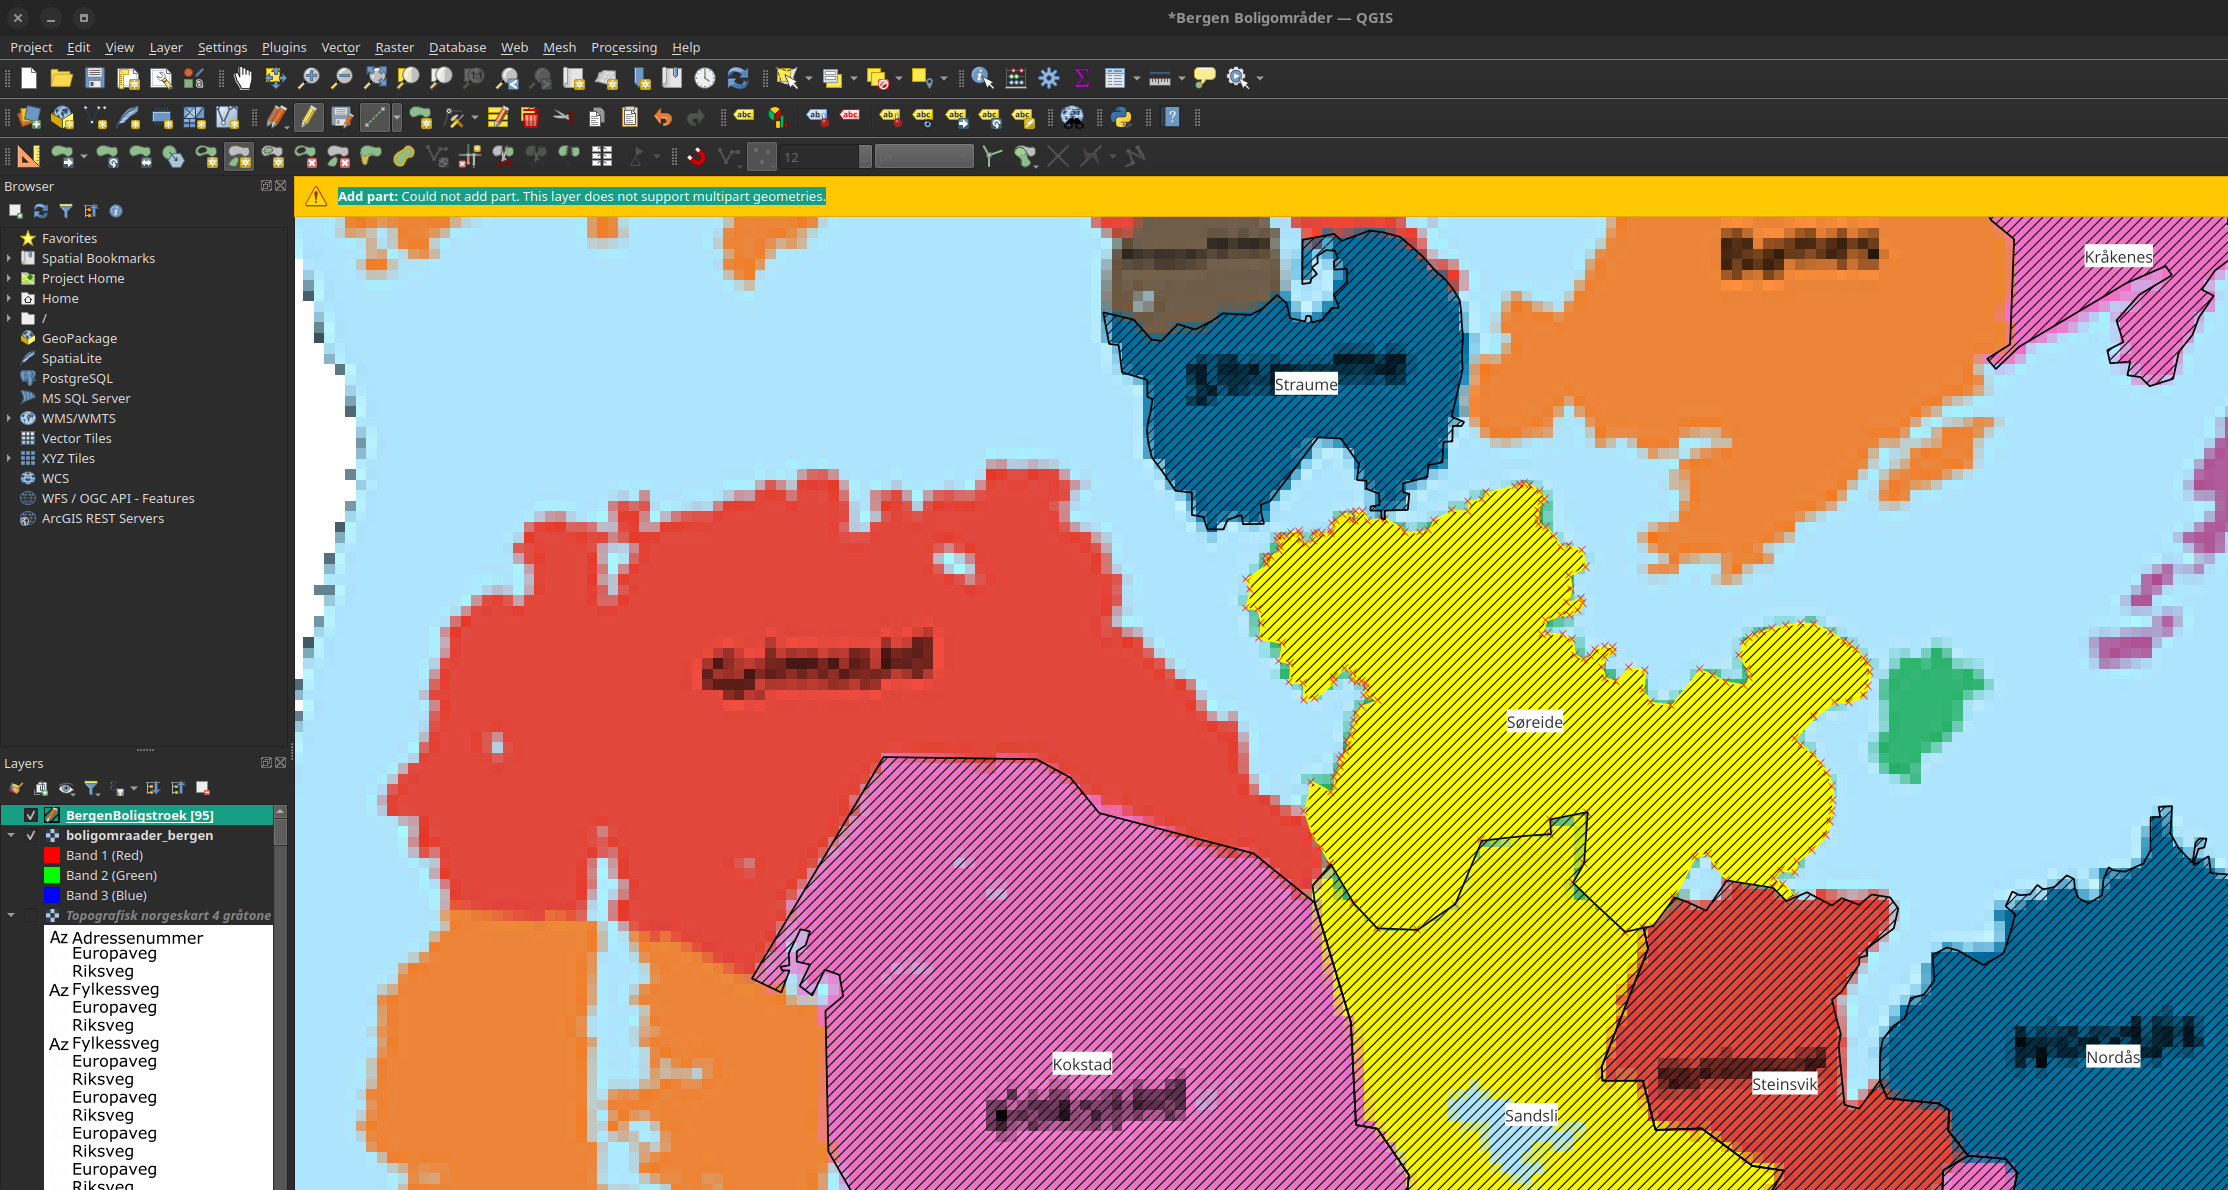
\includegraphics[height = 6cm]{images/qgis_multipart.png}%
%        \caption{}
%    \end{figure}
%\end{frame}

% ====================================
\subsection{Export}
\begin{frame}
    \begin{figure}
        \centering
        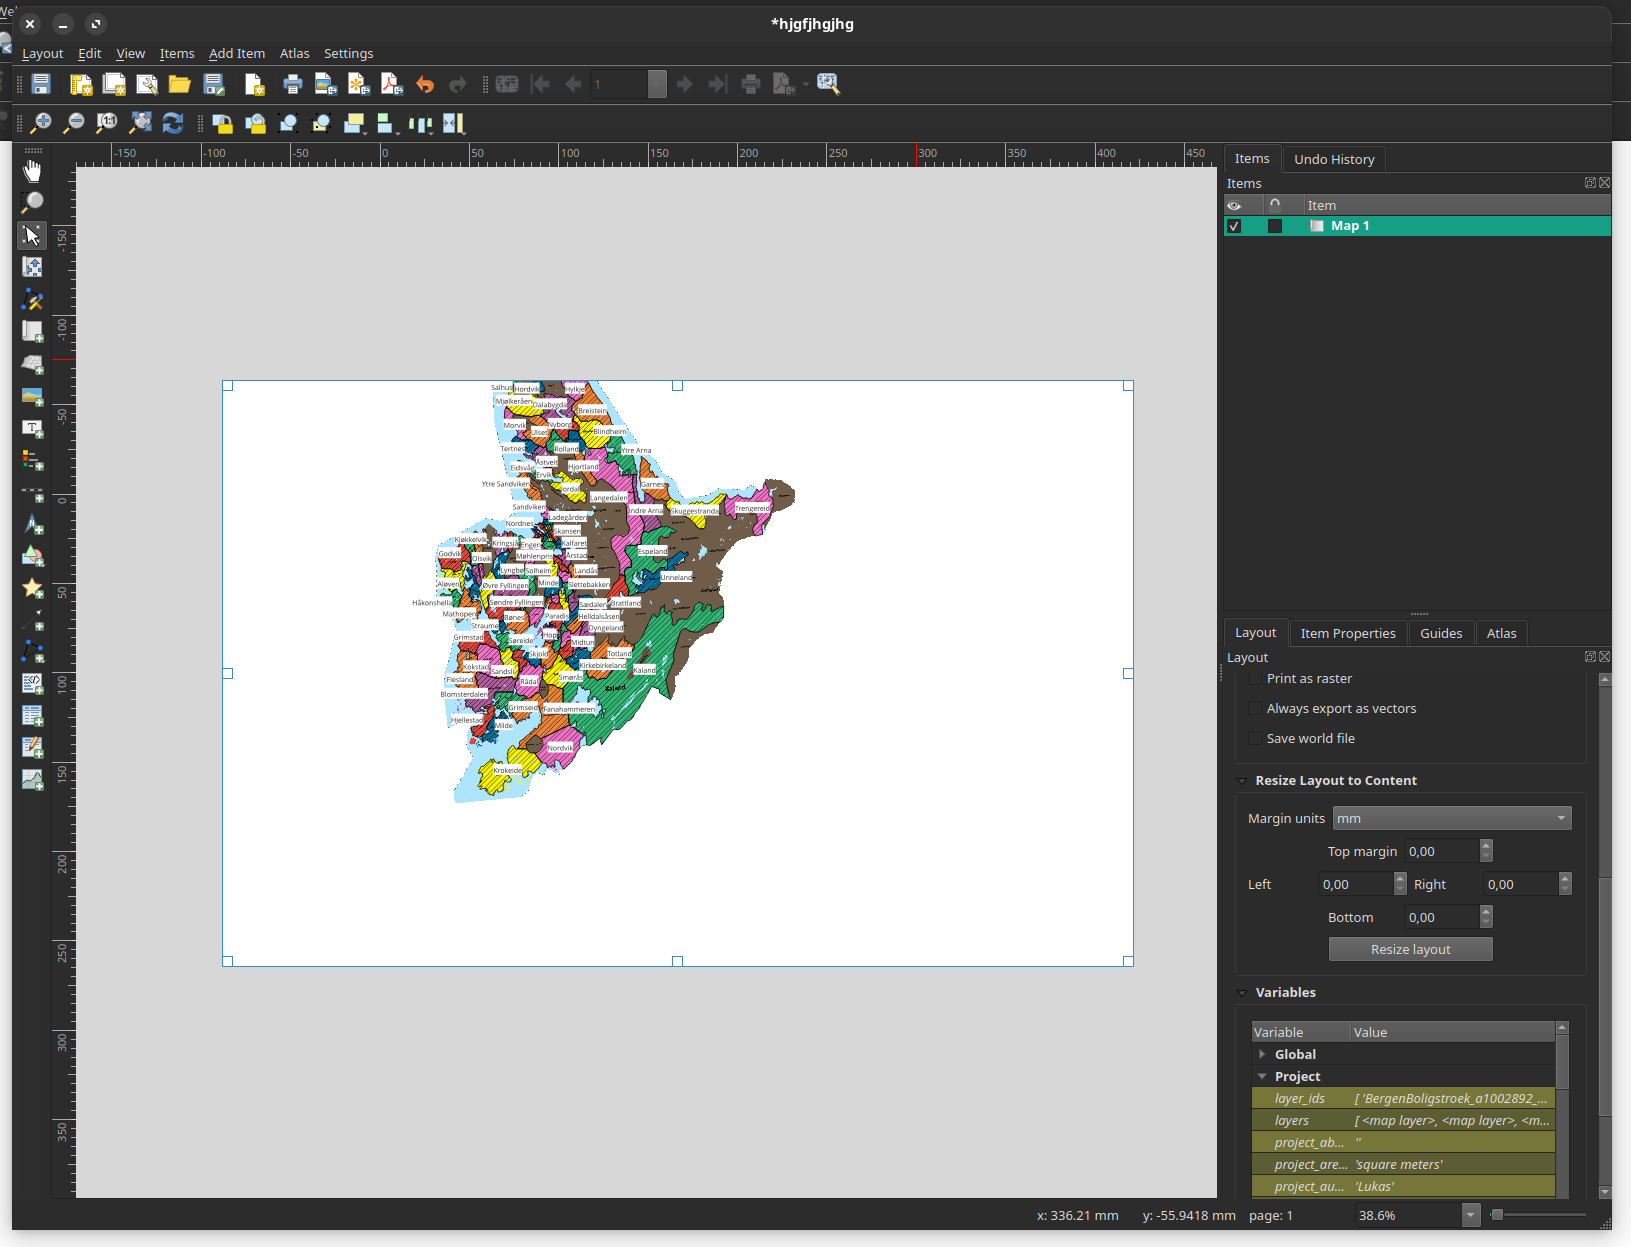
\includegraphics[height = 6cm]{images/qgis_export.png}%
        \caption{Ka e det?}
    \end{figure}
\end{frame}

\begin{frame}
    \begin{block}{Stackoverflow}
        \enquote{You have to select \textit{Vector Data Management Tools Split Vector Layer} on page 4 of the print menu. This will give you one SVG for the entire area and then you can dismantle the SVG file.}
    \end{block}
\end{frame}


\begin{frame}
    \begin{figure}
        \centering
        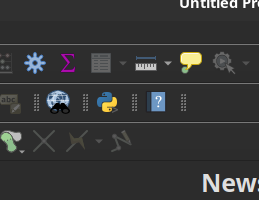
\includegraphics[height = 6cm]{images/qgis_python.png}%
        \caption{Insert Python?}
    \end{figure}
\end{frame}

\begin{frame}
    \begin{figure}
        \centering
        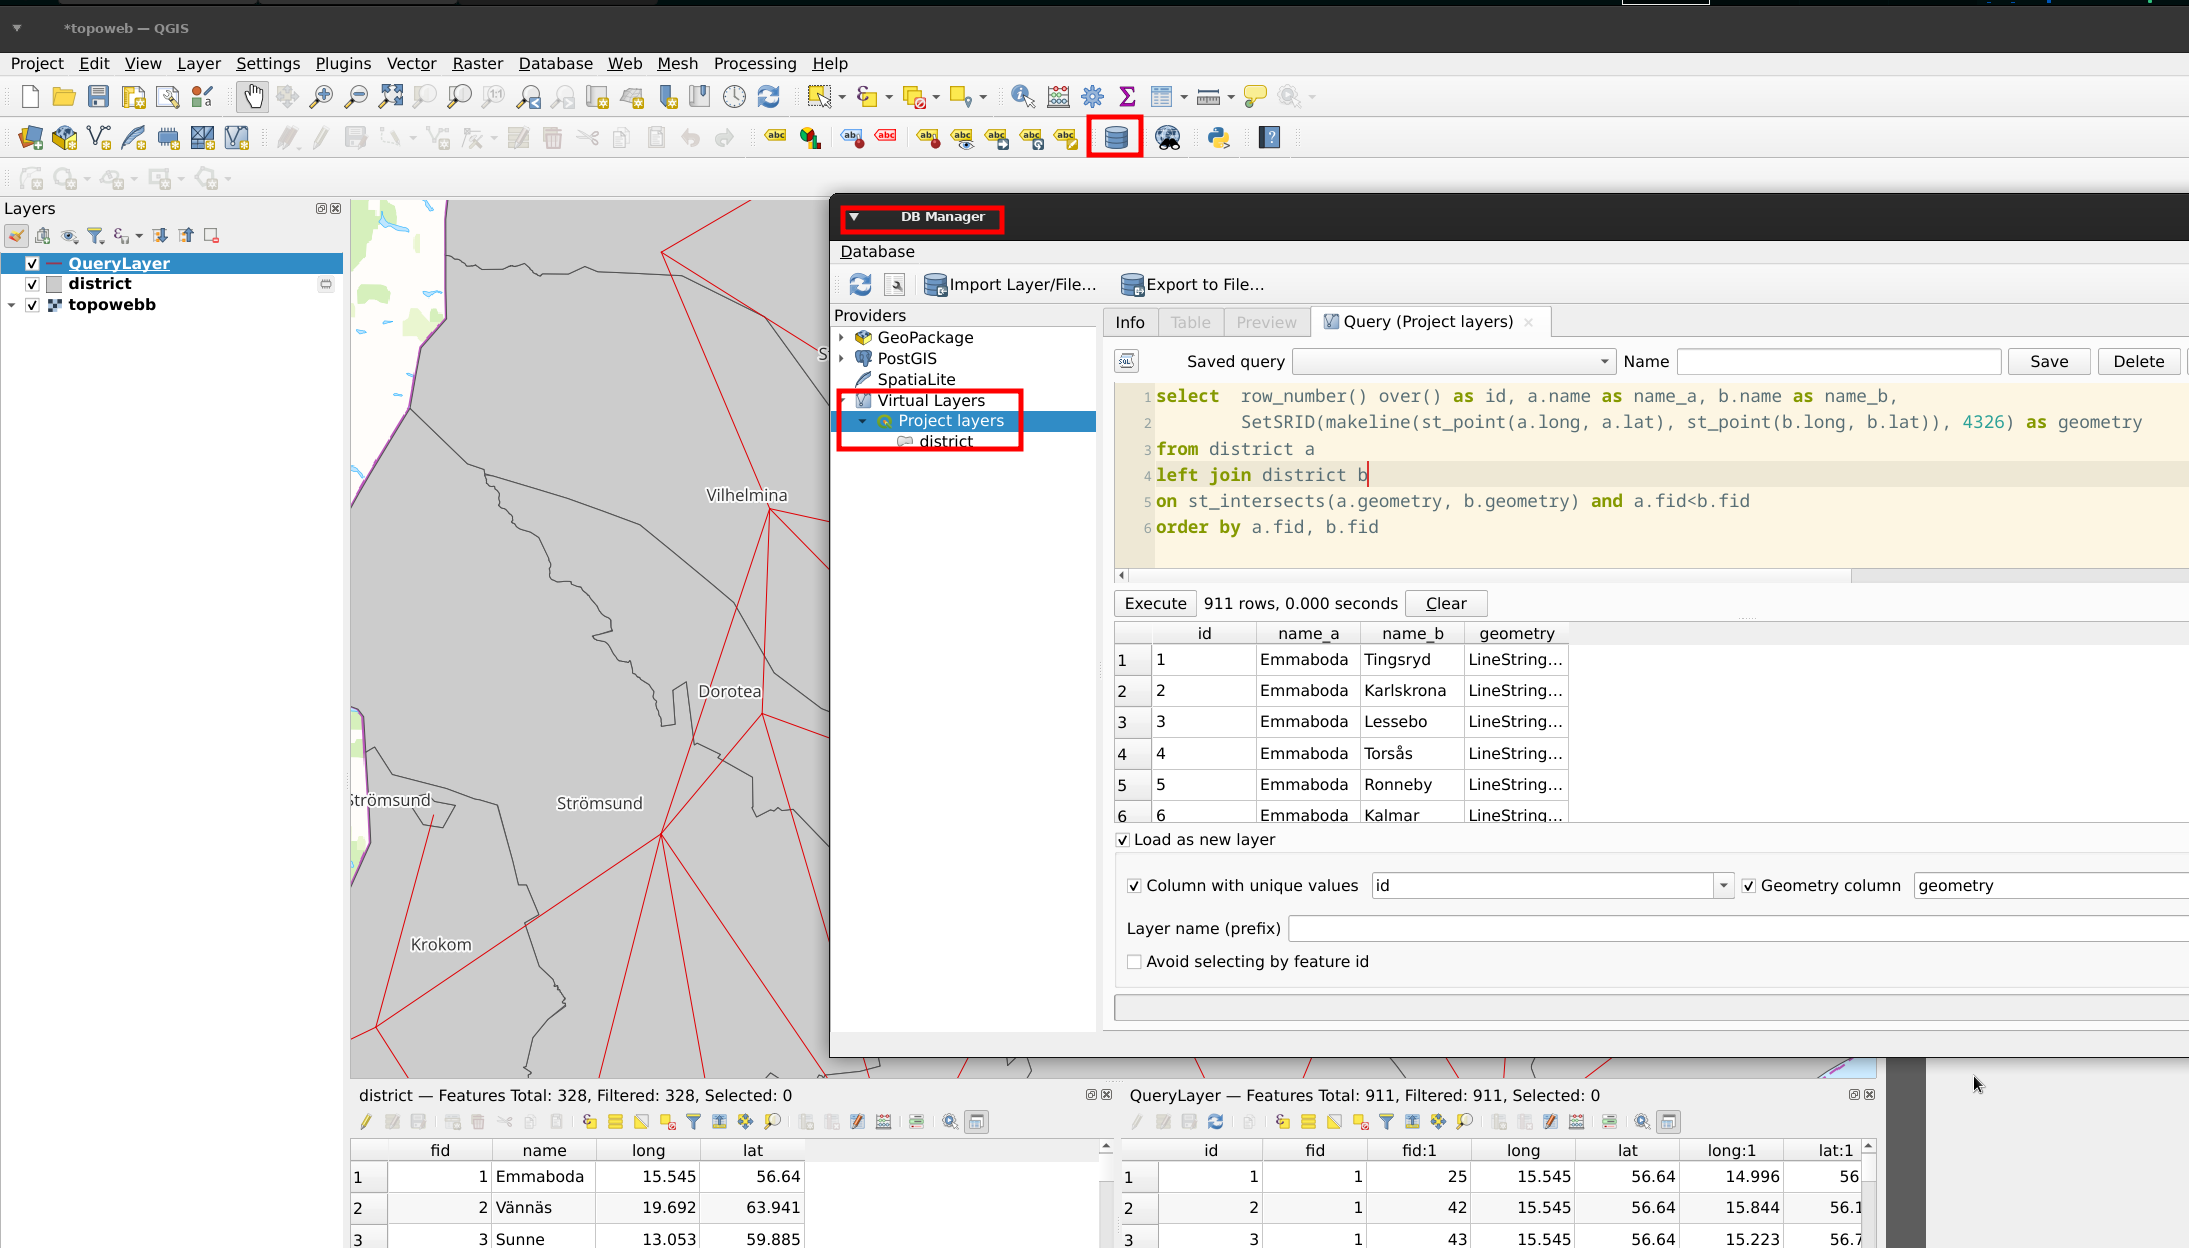
\includegraphics[height = 6cm]{images/qgis_sql.png}%
        \caption{Inline SQL}
    \end{figure}
\end{frame}

\begin{frame}
    \begin{figure}
        \centering
        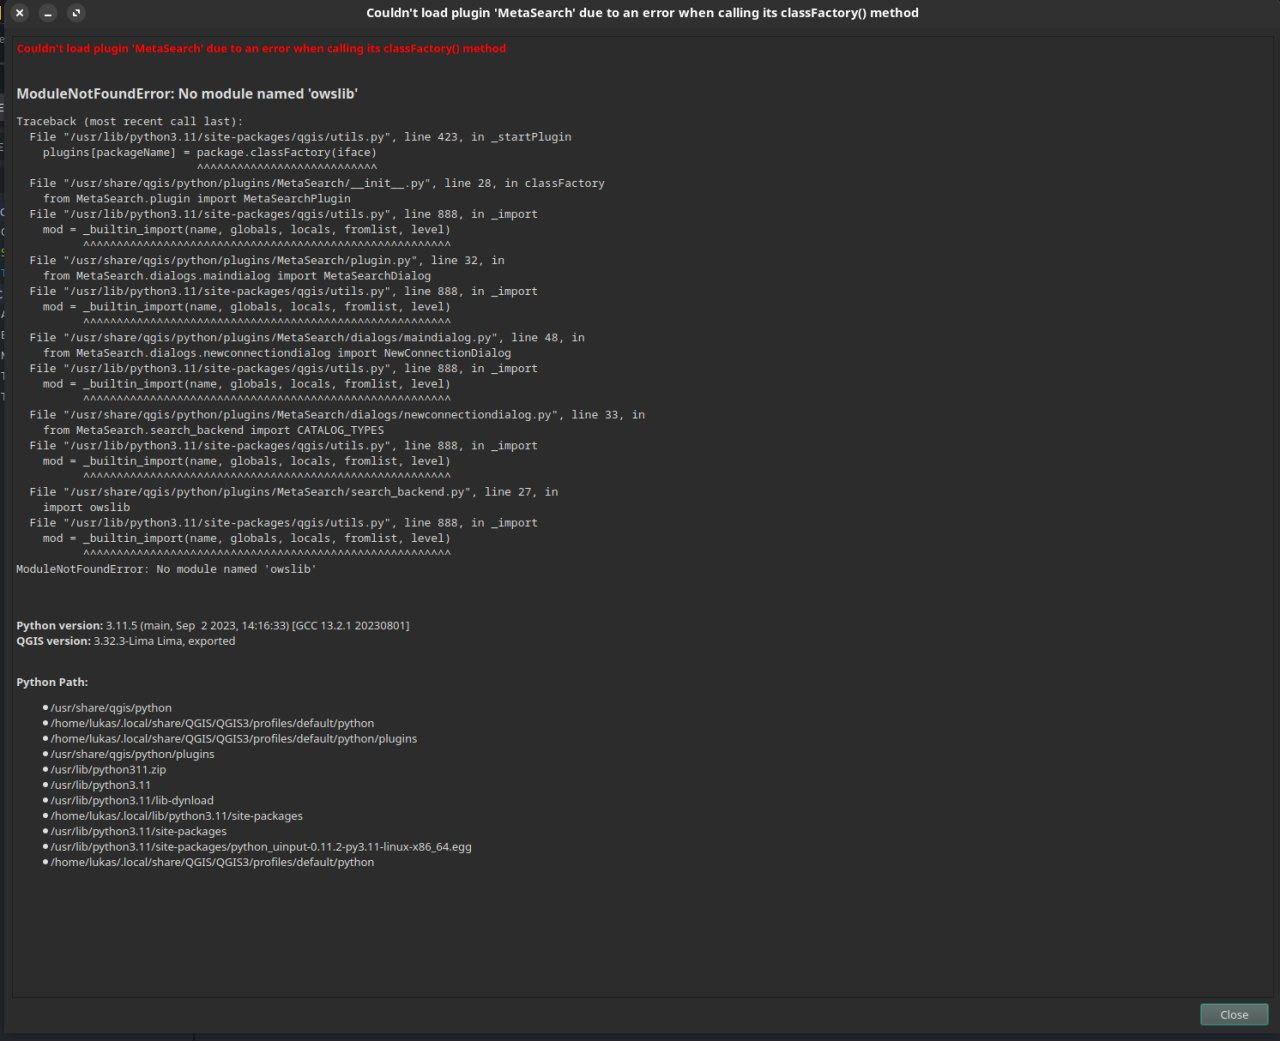
\includegraphics[height = 6cm]{images/qgis_pythonerror.jpg}%
        \caption{Python-Error}
    \end{figure}
\end{frame}

\begin{frame}
    \begin{figure}
        \centering
        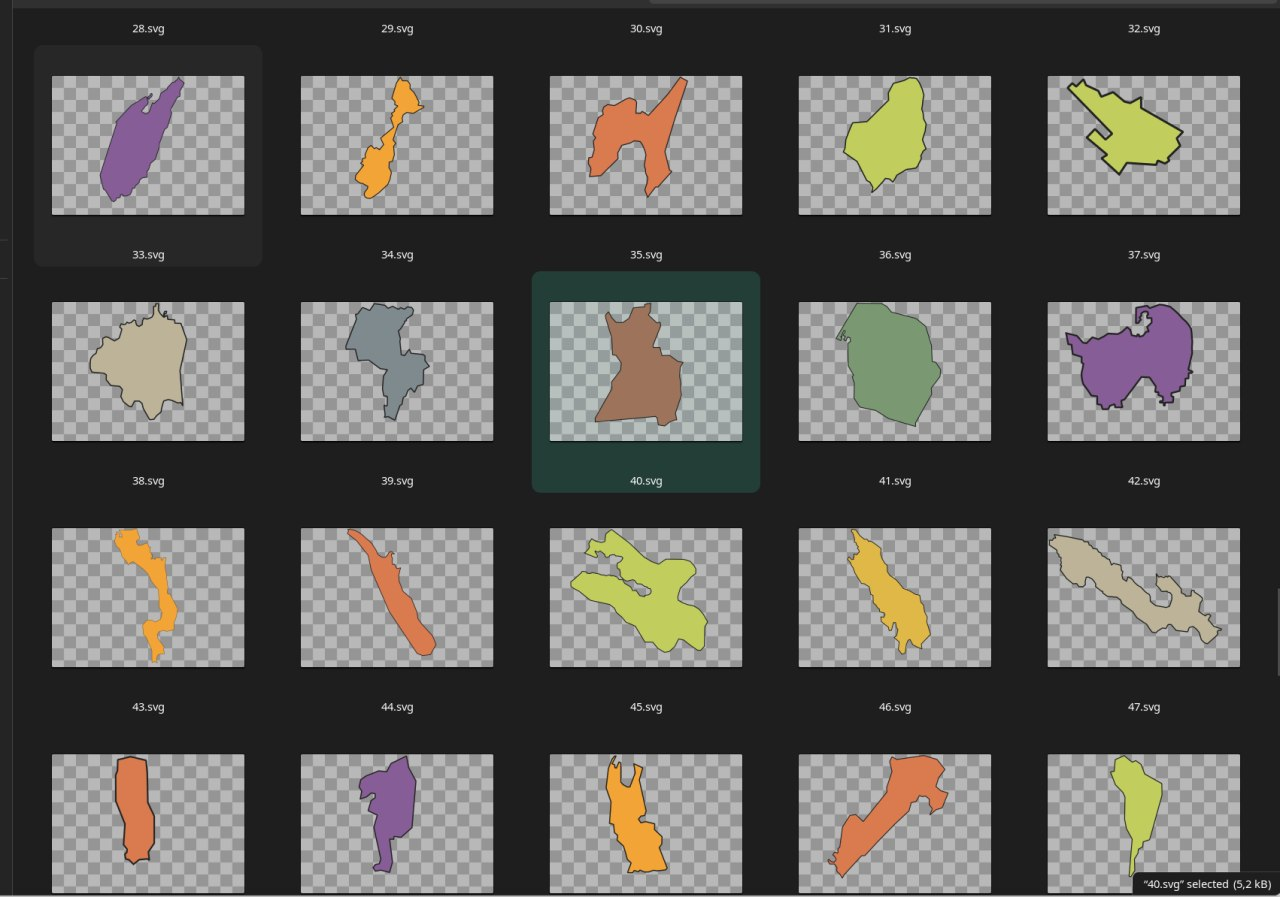
\includegraphics[height = 6cm]{images/svg_finished.jpg}%
        \caption{Finally!}
    \end{figure}
\end{frame}

\begin{frame}
    \begin{figure}
        \centering
        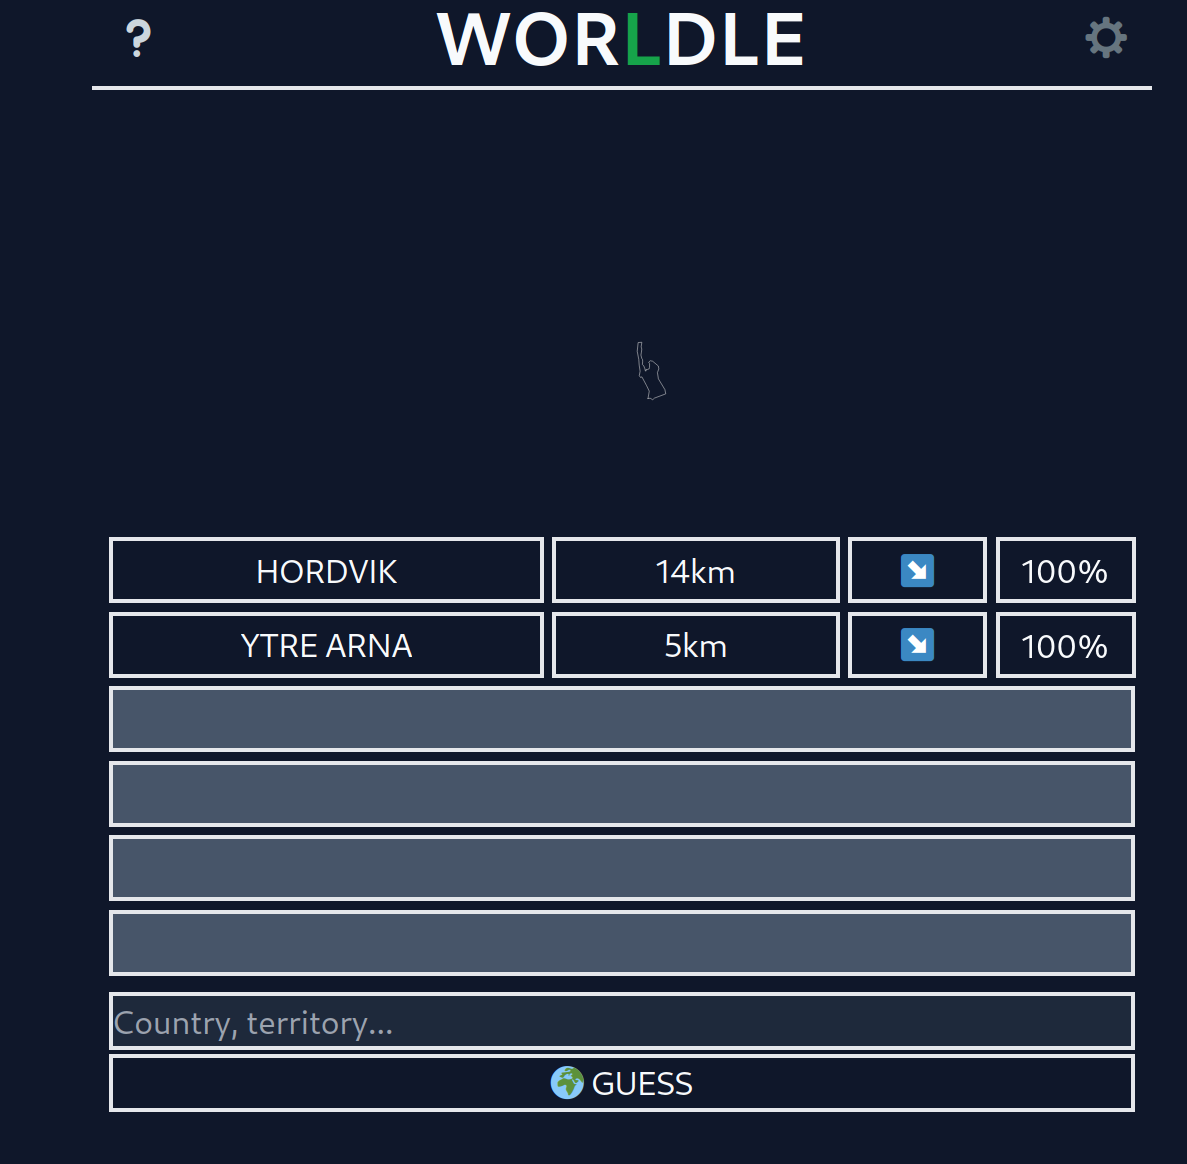
\includegraphics[height = 6cm]{images/svg_toosmall.png}%
        \caption{Wrong SVG-file sizes}
    \end{figure}
\end{frame}

\subsection{Finished website}
\begin{frame}
    \begin{figure}
        \centering
        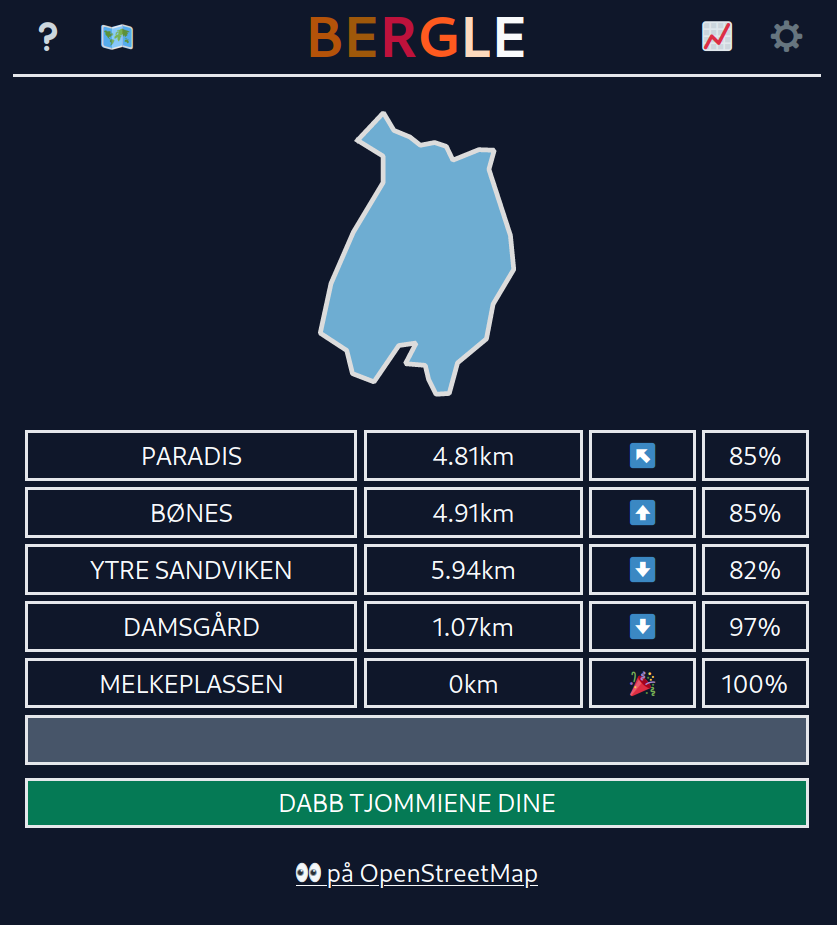
\includegraphics[height = 6cm]{images/bergleFinal.png}%
        \caption{Bergle}
    \end{figure}
\end{frame}

\subsection{Map function}
\begin{frame}
    \begin{figure}
        \centering
        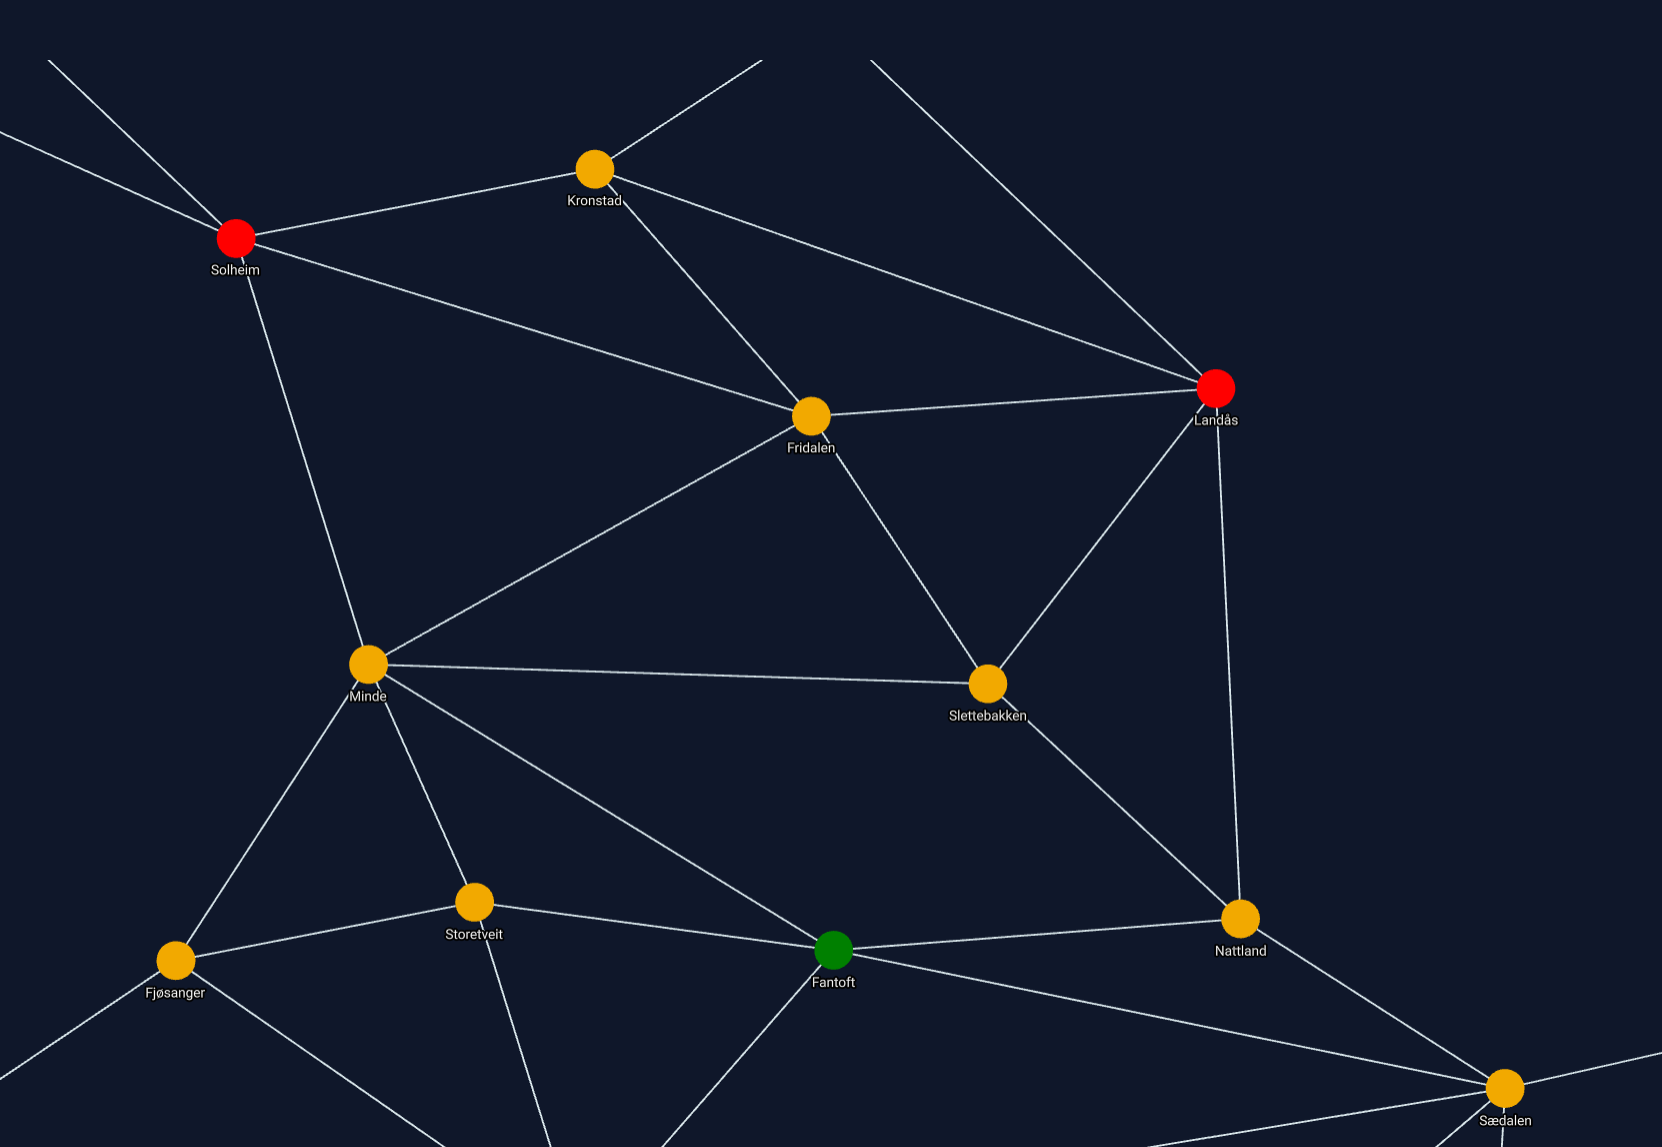
\includegraphics[height = 6cm]{images/map.png}%
        \caption{New map helper function (beta!)}
    \end{figure}
\end{frame}

\subsection{Compass function}
\begin{frame}
    \begin{columns}[t]
        \begin{column}{.4\textwidth}
        \vspace{-0.5cm}
        \hspace{-3cm}
            \begin{figure}
                \centering
                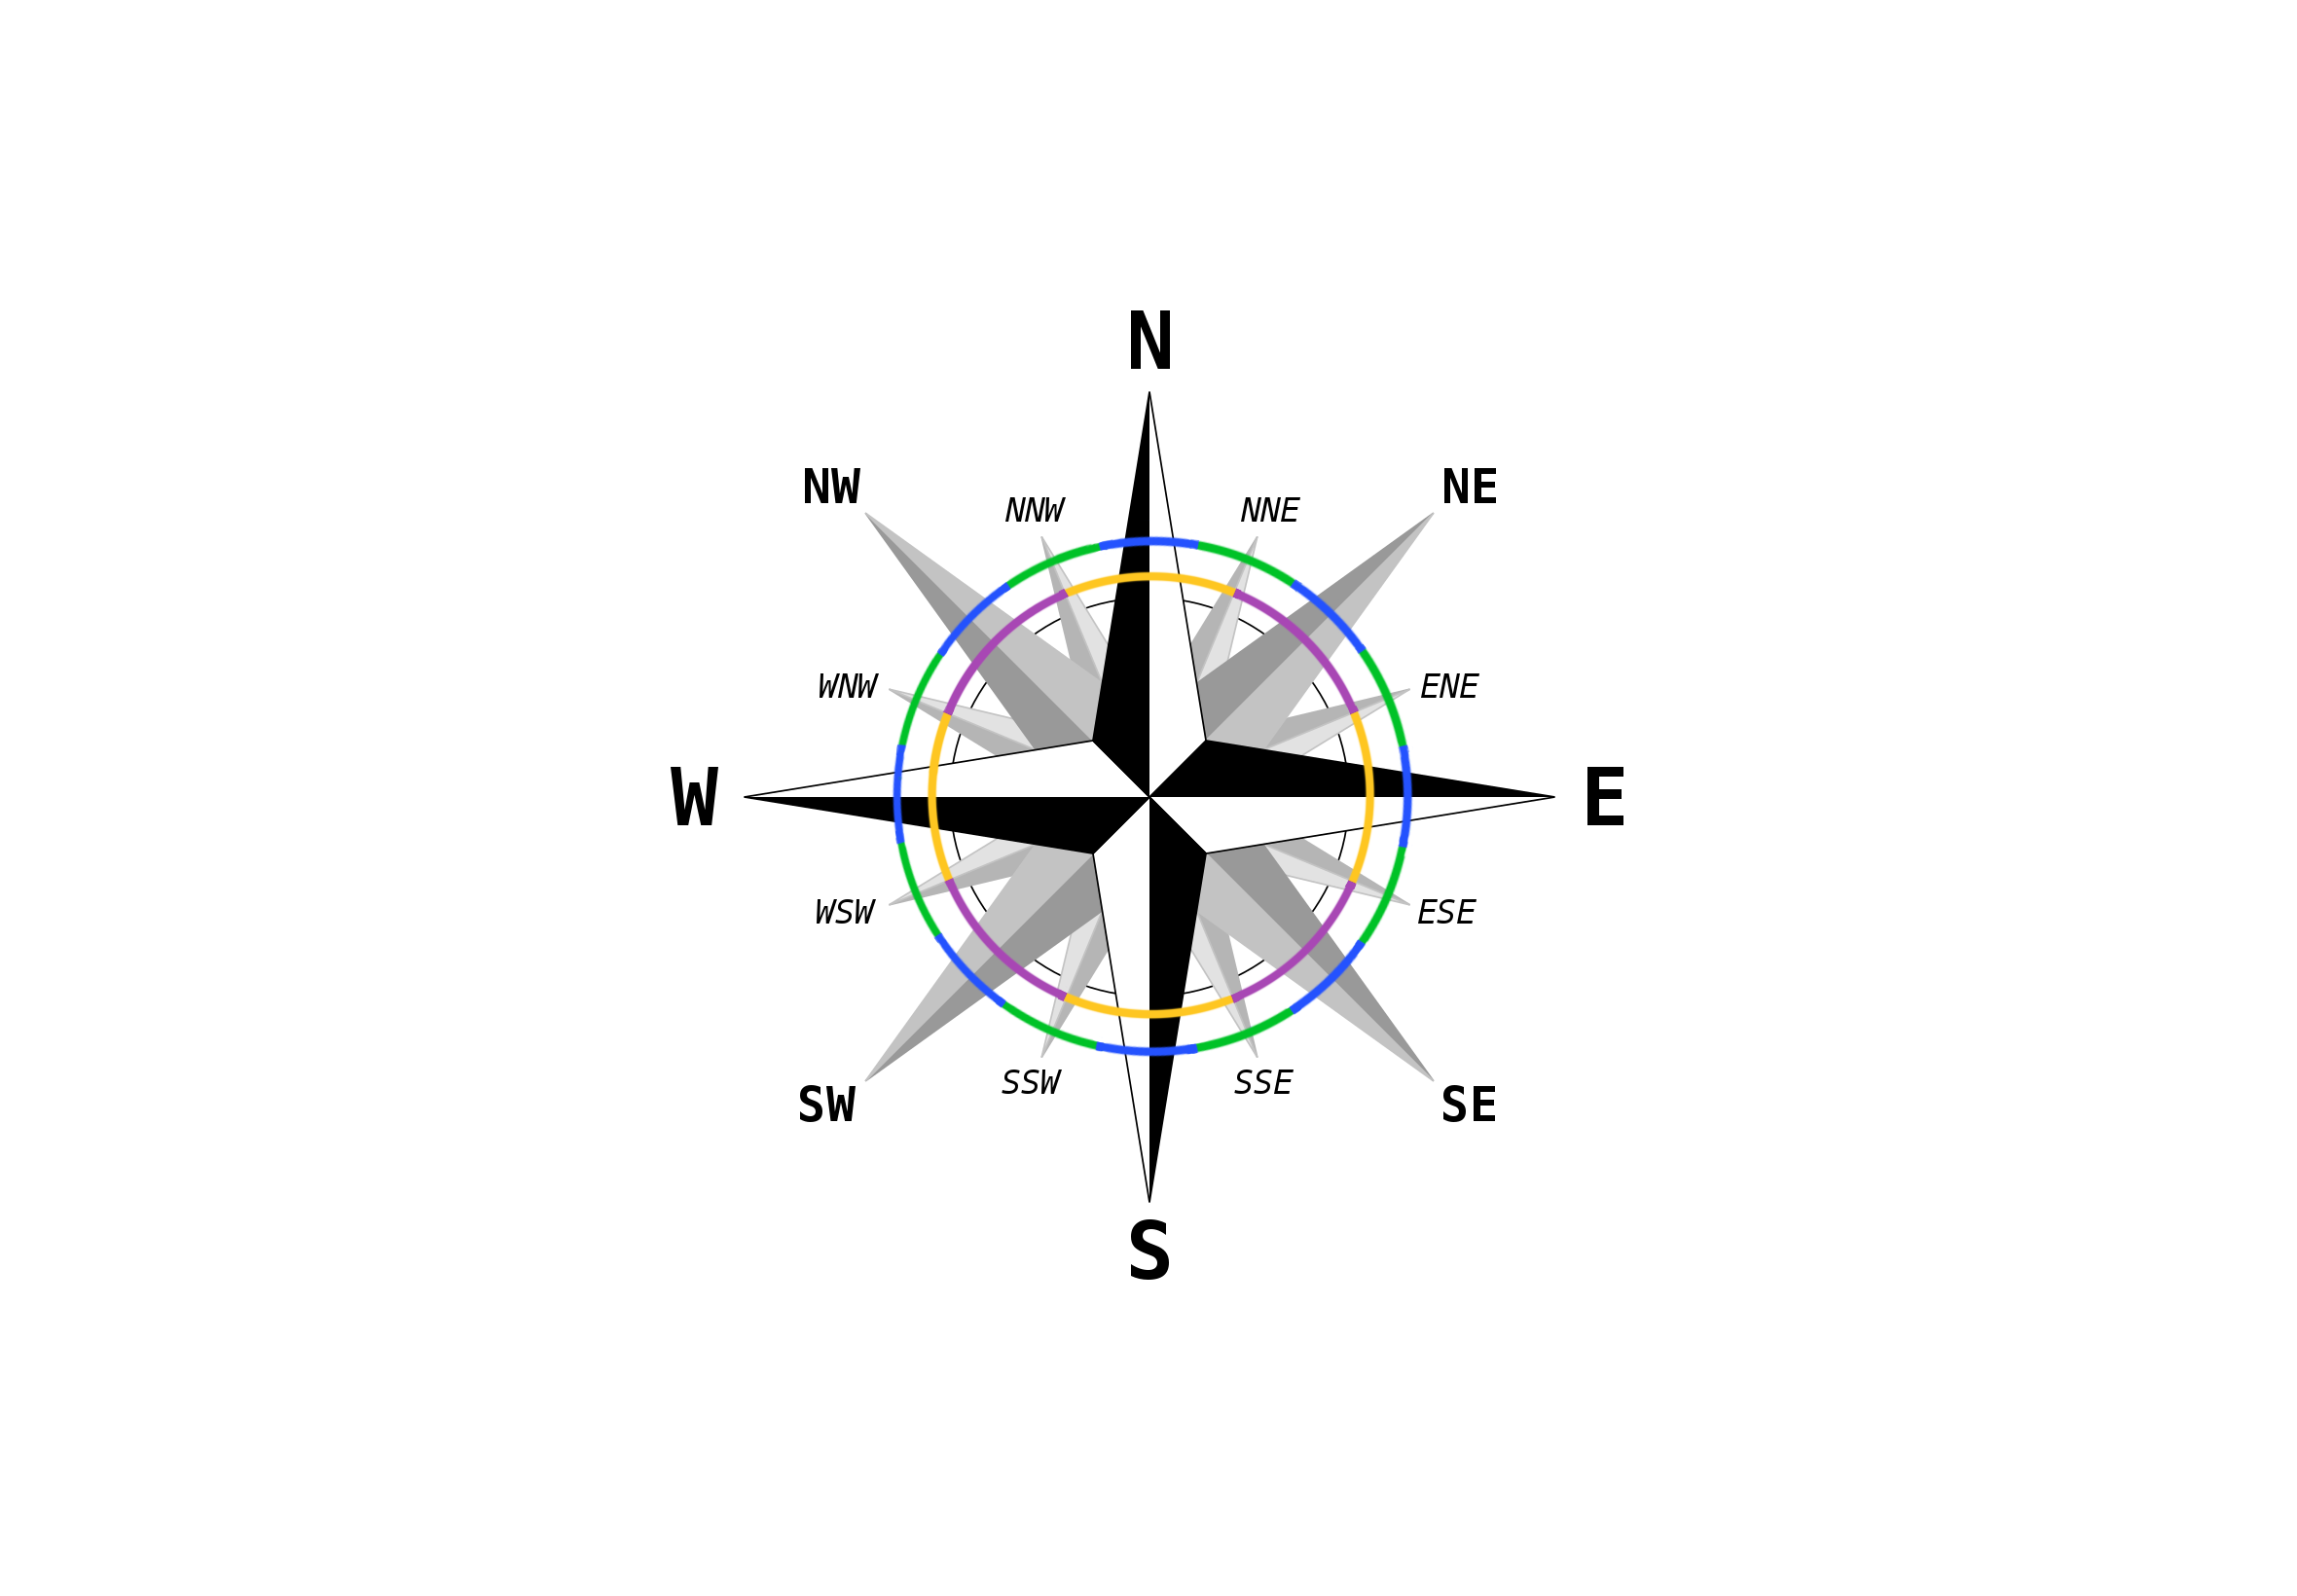
\includegraphics[height = 7cm]{images/compass.png}%
            \end{figure}
        \end{column}
        \hspace{1cm}
        \begin{column}{.6\textwidth}
            \vspace{0.5cm}
            \begin{figure}
                \centering
                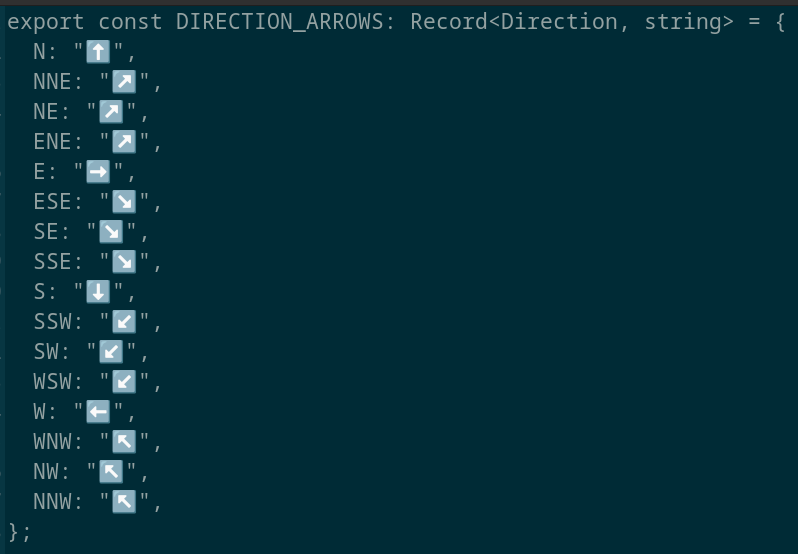
\includegraphics[height = 5cm]{images/directionCode.png}%
            \end{figure}
        \end{column}
    \end{columns}
    
\end{frame}

\section{Angry bergensers}
\begin{frame}
    \begin{block}{Angry bergenser 1}
        But Steinsvik is not it's own area.
    \end{block}
    \pause
    \begin{block}{Angry bergenser 2}
        I do not agree with the border between Fantoft and Paradis, it should be located 50 metres more north.
    \end{block}
    \pause
    \begin{block}{Angry bergenser 3}
        Drotningsvik is missing, it is not part of Godvik!
    \end{block}
\end{frame}

\begin{frame}
    \begin{block}{Angry bergenser 4}
        Fjøsanger was a part of the old city of Fana until 1972, we cannot accept that its now part of the Årstad district, it's Fana!
    \end{block}
    \pause
    \begin{block}{Angry bergenser 5}
        Melkeplassen is not a part of Laksevåg, it is divided equally between Laksevåg and Fyllingsdalen.
    \end{block}
    \pause
    \begin{block}{Angry bergenser 6}
        Bybanen must not go over Bryggen.
    \end{block}
\end{frame}


% Do your audience a favour and let them download the presentation in the beginning
% the QR code file is in the images/-folder
\subsection*{Download Bergle}
\begin{frame}{Scan me}
    \begin{figure}
        \begin{subfigure}{0.45\textwidth}
            \centering
            
\includegraphics[height=4.9cm]{images/bergleqr.png}
            \caption{Bergle}
            \label{fig:qrcodebergle}
        \end{subfigure}
        \hfill
        \begin{subfigure}{0.45\textwidth}
            \centering
            
\includegraphics[height=4.9cm]{images/osloleqr.png}
            \caption{Oslole}
            \label{fig:qrcodeoslole}
        \end{subfigure}
    \end{figure}
\end{frame}

%===============================================

% This is the final slide
%\section*{End}
\begin{frame}
\begin{center}
\begin{Large}
\textbf{Bergle kan kjøpes til kun 11.1 milliarder NOK}
\end{Large}
\\[0.5cm]
Så lenge Konkurransetilsynet og Konkurranseklageemnda sier ja
\end{center}  
\end{frame}